\documentclass[10pt]{article}
\usepackage{arxiv}
\usepackage[T1]{fontenc}
\usepackage[utf8]{inputenc}
\usepackage{newtxtext}
\usepackage[varvw]{newtxmath}
\usepackage[scaled=0.86]{zi4}
\usepackage[protrusion=true,expansion=true]{microtype}
\usepackage{amsmath,bm}
\usepackage{graphicx}
\usepackage{booktabs,multirow,colortbl,tabularx,array}
\usepackage[table]{xcolor}
\usepackage{tikz}
\usetikzlibrary{arrows.meta,positioning,calc,decorations.pathmorphing,shapes.geometric,fit,backgrounds}
\usepackage{algorithm}
\usepackage[noend]{algpseudocode}
\usepackage{enumitem}
\usepackage[font=small,labelfont=bf,labelsep=period,skip=4pt]{caption}
\usepackage{subcaption}
\usepackage[numbers,sort&compress]{natbib}
\usepackage[skins,breakable]{tcolorbox}
\usepackage{siunitx}
\usepackage{hyperref}
\usepackage[capitalise,noabbrev]{cleveref}
\usepackage{tocloft}
\usepackage[section]{placeins}

\definecolor{ink}{HTML}{1B2333}
\definecolor{navy}{HTML}{1F3A5F}
\definecolor{teal}{HTML}{2A9D8F}
\definecolor{amber}{HTML}{E9A23B}
\definecolor{coral}{HTML}{D1495B}
\definecolor{slate}{HTML}{8A94A6}
\definecolor{mist}{HTML}{E8ECF2}
\definecolor{paper}{HTML}{F6F8FB}
\colorlet{realc}{teal}
\colorlet{simc}{coral}
\colorlet{estc}{amber}
\colorlet{repc}{navy}
\tikzset{
  >={Stealth[length=2mm,width=1.5mm]},
  base/.style={font=\sffamily\scriptsize, align=center, inner sep=2.5pt, text=ink},
  box/.style={base, rectangle, rounded corners=2pt, draw=ink!70, line width=0.45pt, fill=white, minimum height=8.5mm, text width=21mm},
  real/.style={box, path picture={\fill[realc] (path picture bounding box.north west) rectangle ([xshift=1.6pt]path picture bounding box.south west);}},
  sim/.style={box, path picture={\fill[simc] (path picture bounding box.north west) rectangle ([xshift=1.6pt]path picture bounding box.south west);}},
  est/.style={box, path picture={\fill[estc] (path picture bounding box.north west) rectangle ([xshift=1.6pt]path picture bounding box.south west);}},
  rep/.style={box, path picture={\fill[repc] (path picture bounding box.north west) rectangle ([xshift=1.6pt]path picture bounding box.south west);}},
  file/.style={base, rectangle, draw=slate, fill=paper, font=\ttfamily\tiny, minimum height=4.6mm, inner sep=1.8pt},
  flow/.style={->, draw=ink!80, line width=0.55pt},
  flowd/.style={->, draw=slate, line width=0.5pt, dashed},
  lane/.style={draw=none, fill=mist!60, rounded corners=4pt},
  lanelabel/.style={font=\sffamily\tiny\bfseries, text=slate, anchor=north west},
  note/.style={font=\sffamily\tiny, text=ink!80, align=center, inner sep=1pt},
  device/.style={base, rectangle, rounded corners=3pt, draw=ink, line width=0.6pt, fill=white, font=\sffamily\scriptsize},
  irwave/.style={draw=coral, line width=0.6pt, decorate, decoration={snake, amplitude=0.5mm, segment length=1.8mm, post length=1.5mm}},
  cross/.style={draw=coral, line width=1pt},
}
\DeclareRobustCommand{\legendchip}[2]{\tikz[baseline=-0.6ex]\fill[#1] (0,-0.75ex) rectangle (1.6pt,0.95ex);\,{\sffamily\scriptsize #2}}

% Generated by figures/make_numbers.py from the episode data. Do not edit by hand.
\newcommand{\EpisodeName}{team\_03}
\newcommand{\ClipFrames}{286}
\newcommand{\ClipFps}{25}
\newcommand{\ClipSeconds}{11.4}
\newcommand{\ClipW}{960}
\newcommand{\ClipH}{540}
\newcommand{\ClipDancers}{1}
\newcommand{\EvCount}{1{,}994{,}349}
\newcommand{\EvRate}{175.0}
\newcommand{\EvOnFrac}{50.1}
\newcommand{\EvW}{320}
\newcommand{\EvH}{180}
\newcommand{\EvPerPixelSec}{3.04}
\newcommand{\SAvailable}{1}
\newcommand{\DetSZero}{99.2}
\newcommand{\ConfSZero}{0.83}
\newcommand{\TransSZero}{1.000}
\newcommand{\LossSZero}{0}
\newcommand{\DriftSZero}{0.0}
\newcommand{\UnuSZero}{0.567}
\newcommand{\DetSTen}{99.2}
\newcommand{\ConfSTen}{0.82}
\newcommand{\TransSTen}{0.544}
\newcommand{\LossSTen}{46}
\newcommand{\DriftSTen}{6.2}
\newcommand{\UnuSTen}{0.758}
\newcommand{\DetSTwenty}{97.3}
\newcommand{\ConfSTwenty}{0.79}
\newcommand{\TransSTwenty}{0.302}
\newcommand{\LossSTwenty}{70}
\newcommand{\DriftSTwenty}{9.2}
\newcommand{\UnuSTwenty}{0.871}
\newcommand{\DetSThirty}{86.9}
\newcommand{\ConfSThirty}{0.69}
\newcommand{\TransSThirty}{0.171}
\newcommand{\LossSThirty}{83}
\newcommand{\DriftSThirty}{19.3}
\newcommand{\UnuSThirty}{0.863}
\newcommand{\DetSForty}{56.3}
\newcommand{\ConfSForty}{0.45}
\newcommand{\TransSForty}{0.098}
\newcommand{\LossSForty}{90}
\newcommand{\DriftSForty}{50.6}
\newcommand{\UnuSForty}{0.847}
\newcommand{\DetSSixty}{0.3}
\newcommand{\ConfSSixty}{0.00}
\newcommand{\TransSSixty}{0.034}
\newcommand{\LossSSixty}{97}
\newcommand{\DriftSSixty}{160.5}
\newcommand{\UnuSSixty}{0.842}
\newcommand{\CAvailable}{1}
\newcommand{\DetCZero}{100.0}
\newcommand{\ConfCZero}{0.98}
\newcommand{\TransCZero}{1.000}
\newcommand{\LossCZero}{0}
\newcommand{\DriftCZero}{0.0}
\newcommand{\UnuCZero}{0.205}
\newcommand{\DetCTen}{100.0}
\newcommand{\ConfCTen}{0.98}
\newcommand{\TransCTen}{0.551}
\newcommand{\LossCTen}{45}
\newcommand{\DriftCTen}{2.9}
\newcommand{\UnuCTen}{0.610}
\newcommand{\DetCTwenty}{94.8}
\newcommand{\ConfCTwenty}{0.88}
\newcommand{\TransCTwenty}{0.309}
\newcommand{\LossCTwenty}{69}
\newcommand{\DriftCTwenty}{12.7}
\newcommand{\UnuCTwenty}{0.873}
\newcommand{\DetCThirty}{29.4}
\newcommand{\ConfCThirty}{0.22}
\newcommand{\TransCThirty}{0.176}
\newcommand{\LossCThirty}{82}
\newcommand{\DriftCThirty}{55.7}
\newcommand{\UnuCThirty}{0.843}
\newcommand{\DetCForty}{20.3}
\newcommand{\ConfCForty}{0.14}
\newcommand{\TransCForty}{0.102}
\newcommand{\LossCForty}{90}
\newcommand{\DriftCForty}{88.7}
\newcommand{\UnuCForty}{0.840}
\newcommand{\DetCSixty}{0.0}
\newcommand{\ConfCSixty}{0.00}
\newcommand{\TransCSixty}{0.036}
\newcommand{\LossCSixty}{96}
\newcommand{\DriftCSixty}{--}
\newcommand{\UnuCSixty}{0.840}
\newcommand{\SoloSeconds}{15.0}
\newcommand{\SoloFrames}{375}
\newcommand{\SoloW}{1272}
\newcommand{\SoloH}{720}
\newcommand{\SoloScore}{0.567}
\newcommand{\SoloAbove}{0.042}
\newcommand{\TakeASec}{13.1}
\newcommand{\TakeABins}{397}
\newcommand{\TakeAScore}{0.234}
\newcommand{\TakeAAbove}{0.015}
\newcommand{\TakeAEvRate}{170.0}
\newcommand{\TakeAArmRange}{15.4}
\newcommand{\TakeALimit}{10}
\newcommand{\TakeBSec}{11.4}
\newcommand{\TakeBBins}{346}
\newcommand{\TakeBScore}{0.214}
\newcommand{\TakeBAbove}{0.014}
\newcommand{\TakeBEvRate}{178.3}
\newcommand{\TakeBArmRange}{15.3}
\newcommand{\TakeBLimit}{2}
\newcommand{\TakeCSec}{11.4}
\newcommand{\TakeCBins}{346}
\newcommand{\TakeCScore}{0.205}
\newcommand{\TakeCAbove}{0.009}
\newcommand{\TakeCEvRate}{175.0}
\newcommand{\TakeCArmRange}{15.7}
\newcommand{\TakeCLimit}{6}
\newcommand{\TakeDSec}{9.8}
\newcommand{\TakeDBins}{297}
\newcommand{\TakeDScore}{0.205}
\newcommand{\TakeDAbove}{0.003}
\newcommand{\TakeDEvRate}{213.1}
\newcommand{\TakeDArmRange}{13.5}
\newcommand{\TakeDLimit}{0}
\newcommand{\TakeESec}{10.8}
\newcommand{\TakeEBins}{327}
\newcommand{\TakeEScore}{0.199}
\newcommand{\TakeEAbove}{0.003}
\newcommand{\TakeEEvRate}{182.1}
\newcommand{\TakeEArmRange}{12.0}
\newcommand{\TakeELimit}{0}
\newcommand{\SteamRho}{1.175}
\newcommand{\RobotLimitHits}{6}
\newcommand{\RobotFrames}{286}
\newcommand{\RobotFirstMove}{0.0}
\newcommand{\SmoothAlpha}{0.52}
\newcommand{\TPose}{16.1}
\newcommand{\TRobot}{3.21}
\newcommand{\TEvents}{3.37}
\newcommand{\TSteam}{17.34}
\newcommand{\PoseFps}{26.2}
\newcommand{\TSoloPose}{16.8}
\newcommand{\TSoloRobot}{10.6}
\newcommand{\TSoloScore}{7.6}
\newcommand{\TSoloViewer}{4.6}
\newcommand{\TSoloSteam}{174}
\newcommand{\SnoreAvailable}{1}
\newcommand{\SnoreSeconds}{44.6}
\newcommand{\SnoreBpm}{16.2}
\newcommand{\SnoreOnsets}{11}
\newcommand{\SnoreEvRate}{11.5}
\newcommand{\SnoreChannels}{64}
\newcommand{\SnoreTheta}{1.40}
\newcommand{\SnoreCadence}{0.31}
\newcommand{\SnorePauses}{0}
\newcommand{\SnoreEvCount}{513{,}978}

\newcommand{\PhysIter}{500}
\newcommand{\PhysEnvs}{4096}
\newcommand{\PhysSeconds}{13.4}
\newcommand{\PhysBodyErrCm}{3.7}
\newcommand{\PhysJointRmse}{0.17}
\newcommand{\PhysArmRmse}{0.18}
\newcommand{\PhysMinHeight}{0.77}
\newcommand{\PhysUpright}{0.974}
\newcommand{\PhysDrift}{5.4}
\newcommand{\PhysFell}{no}
\newcommand{\PhysTrainMin}{5.4}
\newcommand{\PhysGPU}{NVIDIA B300}


\hypersetup{colorlinks=true, linkcolor=navy, citecolor=teal!80!black, urlcolor=navy, pdftitle={VLMA: Vision-Language-Macarena-Action}, pdfauthor={Artificial Idiocy}}
\renewcommand{\headeright}{NullHacks\{Helsinki\} 2026}
\renewcommand{\undertitle}{Preprint, under review by null overlords.}
\renewcommand{\shorttitle}{VLMA: Vision-Language-Macarena-Action}
\setlength{\cftbeforesecskip}{1.5pt}
\renewcommand{\cftsecfont}{\small\bfseries}
\renewcommand{\cftsubsecfont}{\small}
\renewcommand{\cftsecpagefont}{\small\bfseries}
\renewcommand{\cftsubsecpagefont}{\small}
\setlength{\cftbeforetoctitleskip}{0pt}
\setlength{\cftaftertoctitleskip}{4pt}
\renewcommand{\cfttoctitlefont}{\normalsize\bfseries\sffamily}
\setlist{itemsep=1pt, topsep=3pt, leftmargin=*}
\renewcommand{\topfraction}{0.9}
\renewcommand{\bottomfraction}{0.6}
\renewcommand{\textfraction}{0.08}
\renewcommand{\floatpagefraction}{0.75}
\setcounter{topnumber}{3}
\setcounter{bottomnumber}{2}
\setcounter{totalnumber}{5}
\setlength{\textfloatsep}{12pt plus 2pt minus 4pt}

\newcommand{\vlma}{\textsc{VLMA}}
\newcommand{\realtag}{\emph{real}}
\newcommand{\simtag}{\emph{simulated}}
\newcommand{\esttag}{\emph{estimated}}
\newcommand{\reptag}{\emph{replay}}
\newcommand{\file}[1]{\texttt{#1}}
\newcommand{\R}{\mathbb{R}}
\newcommand{\relu}{\operatorname{relu}}
\newcommand{\nrm}{\operatorname{unit}}
\newcommand{\clip}{\operatorname{clip}}
\sisetup{group-separator={,}, group-minimum-digits=4}

\newtcolorbox{takeaway}[1][]{enhanced, breakable, colback=paper, colframe=navy, boxrule=0pt, leftrule=2pt, arc=0pt, left=6pt, right=6pt, top=4pt, bottom=4pt, fontupper=\small, #1}

\title{\vlma: Vision-Language-Macarena-Action\\[4pt]
\large\mdseries One Phone Clip to a Multi-Sensor Humanoid Dataset,\\ and a Measurement of Where It Breaks in a Finnish Sauna}

\author{
  \textbf{\{Artificial Idiocy\}}\\
  NullHacks\{Helsinki\} 2026\\
  \texttt{github repository linked in the submission}
}
\date{}

\begin{document}
\maketitle

\begin{abstract}
Robots have folded many towels and, to our knowledge, performed no macarenas. \vlma{} is a laptop-only pipeline that turns one phone clip into a time-aligned humanoid episode: an event-camera stream \emph{simulated} from the video, a pose \emph{estimated} by MediaPipe, a Unitree G1 that \emph{replays} the arms in MuJoCo through bounded torso-frame inverse kinematics, and a per-dancer unusualness score from a spiking network calibrated to percentiles of clean dancing. On a public macarena performer held out from training, its author measures a mean of 0.471 against a calibrated 0.5; with models trained in our room, 8 of 9 deliberately bad takes are flagged. We then apply \emph{Finnish onboarding}, a simulated steam veil of rising optical depth. Pose tracking holds at \DetSTwenty\% of frames at level 20 ($\bar T=\TransSTwenty$), falls to \DetSForty\% at level 40 and to \DetSSixty\% at level 60, while the mean unusualness score rises from \UnuSZero{} to \UnuSTwenty{} by level 20: the scorer notices the steam before the tracker fails. A simulated silicon cochlea on a real snore adds a breathing cadence of \SnoreBpm{} per minute. The episode runs on one CPU in one command. Finally, a reinforcement-learning tracking policy trained in about \PhysTrainMin{} minutes on one GPU makes the G1 dance our take in full rigid-body physics: \PhysSeconds\,s without a fall, within \PhysBodyErrCm\,cm of the reference per body.
\end{abstract}

\keywords{event cameras \and spiking neural networks \and humanoid retargeting \and robustness \and sauna \and macarena}

\vspace{6pt}
\begin{takeaway}
\textbf{What is real in this paper.} The phone video and the snoring audio are real recordings. Pose is estimated by MediaPipe. Events, steam and the cochlea are simulated. The humanoid replay is kinematic; the physics policy of \cref{sec:physics} balances and applies torques, but only in simulation, never on a real robot. The spiking scorer was trained by a teammate on 21 clean clips, 16 public videos and our five cabin takes. Every number comes from a file written by the pipeline (\cref{app:repro}).
\end{takeaway}

\clearpage
{\small\tableofcontents}
\vspace{4pt}
{\small\listoffigures}

\clearpage
\begin{figure}[t]
  \centering
  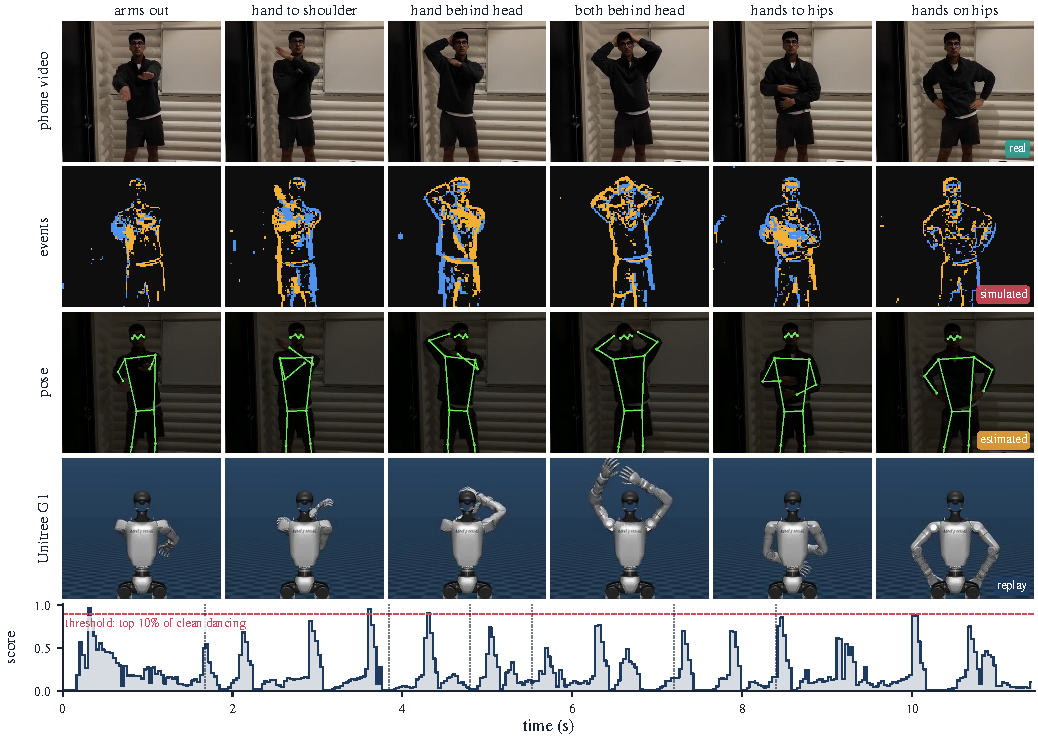
\includegraphics[width=\linewidth]{figures/out/teaser.pdf}
  \caption[One macarena, four streams, one command]{\textbf{One macarena, four streams, one command.} Six moves from cabin take 3 (\TakeCSec\,s, \ClipFps\,fps), filmed by the team. Rows: the \emph{real} phone video; events \emph{simulated} from it (ON amber, OFF blue, 100\,ms window); the \emph{estimated} COCO-17 skeleton; the Unitree G1 in MuJoCo as a kinematic \emph{replay} of that pose. Bottom: the spiking scorer's unusualness per 33\,ms bin, a percentile of clean dancing by other dancers; dotted lines mark the six frames. Tiles are cropped to the dancer.}
  \label{fig:teaser}
\end{figure}

\section{Introduction}
\label{sec:intro}

Vision-language-action models map pixels and instructions to robot actions~\cite{brohan2023rt2,kim2024openvla,black2024pi0}, and are trained on corpora of objects being picked, placed and folded. There is no ImageNet of the macarena~\cite{losdelrio1993macarena}. Human-to-humanoid motion work closes much of the gap for general motion~\cite{shen2024gvhmr,araujo2025gmr,peng2018deepmimic}, but assumes a GPU, a parametric body model~\cite{loper2015smpl} and a motion-capture archive~\cite{mahmood2019amass}. We ask a smaller question: what is the cheapest credible path from a phone clip of a dance to a robot-ready, multi-sensor episode, and where does it break?

The output is one folder per clip with a fixed contract (\cref{fig:schema}): source video, simulated events, estimated pose, humanoid replay, unusualness score and a combined video for a television. The setting is a log cabin on the Finnish coast, so the robustness test is the sauna. The steam is simulated; the tracker's response to it is measured.

\paragraph{Contributions.}
\begin{enumerate}[label=\textbf{C\arabic*.}]
  \item \textbf{A one-command, CPU-only pipeline} (\cref{alg:run}) from a phone clip to an episode folder with five aligned streams, each labelled real, estimated, simulated or replayed (\cref{tab:realsim}), run on five real macarena takes.
  \item \textbf{A torso-frame retargeting} of estimated 3D landmarks onto the Unitree G1 arms by bounded nonlinear least squares against the robot's own forward kinematics, with no hard-coded source axes (\cref{sec:ik}).
  \item \textbf{An event-based unusualness scorer}: 26 event features per dancer per 33\,ms bin, a two-layer spiking network adapted from a previous project with on/off encoding, adaptive thresholds and top-$k$ inhibition, and percentile calibration, evaluated against a Mahalanobis baseline, with a negative result on STDP and on transfer to new dancers (\cref{sec:scorer,sec:exp-scorer}).
  \item \textbf{Finnish onboarding}, a reproducible steam-veil robustness sweep grounded in Koschmieder's law, with a measured failure curve for pose tracking on a real macarena (\cref{sec:steam,sec:exp-steam}).
  \item \textbf{Robot ears}: a simulated silicon cochlea that turns real audio into address events and a breathing estimate (\cref{sec:ears,sec:exp-ears}).
  \item \textbf{From replay to physics}: a whole-body tracking policy, trained by PPO on \PhysEnvs{} parallel simulated G1s, that performs our take with balance, contacts and torque limits (\cref{sec:physics,sec:exp-physics}).
\end{enumerate}

\section{Related Work}
\label{sec:related}

\paragraph{Vision-language-action models.} RT-2~\cite{brohan2023rt2}, OpenVLA~\cite{kim2024openvla} and $\pi_0$~\cite{black2024pi0} map images and language to actions with large pretrained backbones. \vlma{} contains no language model; the L stands for a single, culturally fixed instruction, which removes the need for one.

\paragraph{Human motion to humanoids.} GVHMR~\cite{shen2024gvhmr} recovers world-grounded human motion from monocular video; GMR~\cite{araujo2025gmr} shows that retargeting quality matters for humanoid motion tracking; DeepMimic~\cite{peng2018deepmimic} learns physics-based controllers that imitate reference motion. These systems use SMPL~\cite{loper2015smpl} bodies and AMASS-scale data~\cite{mahmood2019amass}. Ours is deliberately smaller: per-frame landmark directions matched to the robot's forward kinematics in MuJoCo~\cite{todorov2012mujoco} with the Menagerie G1 model~\cite{menagerie2022,unitreeg1}, no body model, and no dynamics. It is a kinematic replay, not a controller.

\paragraph{Pose estimation.} We use the MediaPipe~\cite{lugaresi2019mediapipe} Pose Landmarker, descended from BlazePose~\cite{bazarevsky2020blazepose}, which predicts 33 landmarks with metric world coordinates on a CPU. We export the COCO-17 subset~\cite{lin2014coco} used by OpenPose-style tools~\cite{cao2021openpose}.

\paragraph{Event cameras and their simulation.} Dynamic vision sensors report per-pixel log-intensity changes asynchronously~\cite{lichtsteiner2008dvs,brandli2014davis}; see~\cite{gallego2022survey} for a survey. Since event hardware is scarce, simulators convert video into events: ESIM~\cite{rebecq2018esim}, the simulator of Mueggler et al.~\cite{mueggler2017dataset}, Video to Events~\cite{gehrig2020video2events} and v2e~\cite{hu2021v2e}, which also models noise and finite bandwidth. Our events come from eventify, an idealised frame-difference simulator the team wrote earlier, and are stored in the DVS128 Gesture layout~\cite{amir2017gesture}. We claim no sensor realism beyond the idealised model.

\paragraph{Spiking networks and STDP.} Spiking networks~\cite{maass1997spiking,gerstner2002spiking} compute with leaky integrate-and-fire neurons. Spike-timing-dependent plasticity~\cite{bi1998stdp} with lateral inhibition and adaptive thresholds learns features without labels~\cite{diehl2015unsupervised}. We use snnTorch-style LIF dynamics~\cite{eshraghian2023snntorch} and report that, in our setting, STDP does not specialise the weights.

\paragraph{Anomaly scoring.} Distance to a fitted Gaussian~\cite{mahalanobis1936} is a classic novelty detector~\cite{chandola2009anomaly}; template alignment by dynamic time warping~\cite{sakoe1978dtw} is the classic alternative for motion. We use the Mahalanobis distance as the baseline the spiking network has to beat.

\paragraph{Vision through scattering media.} Koschmieder's law~\cite{koschmieder1924} models a scene seen through haze as attenuated radiance plus airlight; Narasimhan and Nayar~\cite{narasimhan2002vision} and the dark channel prior~\cite{he2009dark} build on it. Domain randomisation~\cite{tobin2017domain} perturbs rendering to harden perception. We use the model the other way round: to break a tracker in a controlled, reproducible way.

\paragraph{Neuromorphic audition.} Silicon cochleae~\cite{lyon1988cochlea} split sound into frequency channels; AER EAR~\cite{chan2007aerear} and the Dynamic Audio Sensor~\cite{liu2014das} emit address events per channel. Our cochlea is a software simulation inspired by these designs, not a model of any chip.

\section{System Overview}
\label{sec:overview}

\Cref{fig:pipeline} shows the four lanes of the pipeline and \cref{fig:hardware} the deployment. A phone clip enters on the left. Lane A simulates events and scores each dancer; lane B estimates pose and replays it on the G1; lane C re-runs pose under simulated steam; lane D listens. All lanes write into one episode folder (\cref{fig:schema}) and a viewer composes a labelled $2{\times}2$ panel with a score strip for the TV. \Cref{alg:run} is the one command.

\paragraph{Problem statement.} Given a clip $V=(I_1,\dots,I_F)$ at frame rate $f_s$ with $D\le3$ dancers, \vlma{} computes the episode
\begin{equation}
  \mathcal{E}(V) = \Big(\,V,\; \underbrace{\{(x_j,y_j,t_j,p_j)\}_{j=1}^{M}}_{\text{simulated events}},\; \underbrace{\mathbf{K}\in\R^{F\times D\times17\times3}}_{\text{estimated pose}},\; \underbrace{q_{1:F}\in\mathcal{Q}^{F}}_{\text{kinematic replay}},\; \underbrace{\mathbf{s}\in[0,1]^{B\times D}}_{\text{unusualness}}\Big),
  \label{eq:episode}
\end{equation}
where $\mathcal{Q}=\prod_i[q_i^{\min},q_i^{\max}]$ is the G1's joint box and $B=\lceil 1000F/(33f_s)\rceil$ is the number of 33\,ms bins. Each component is a deterministic function of $V$ and a fixed seed. Under the steam operator $\mathcal{T}_\ell$ of \cref{sec:steam} we measure how far $\mathbf{K}$ and $\mathbf{s}$ move, $\mathcal{E}(\mathcal{T}_\ell V)$ against $\mathcal{E}(V)$.

\begin{figure}[tbp]
  \centering
  \resizebox{\linewidth}{!}{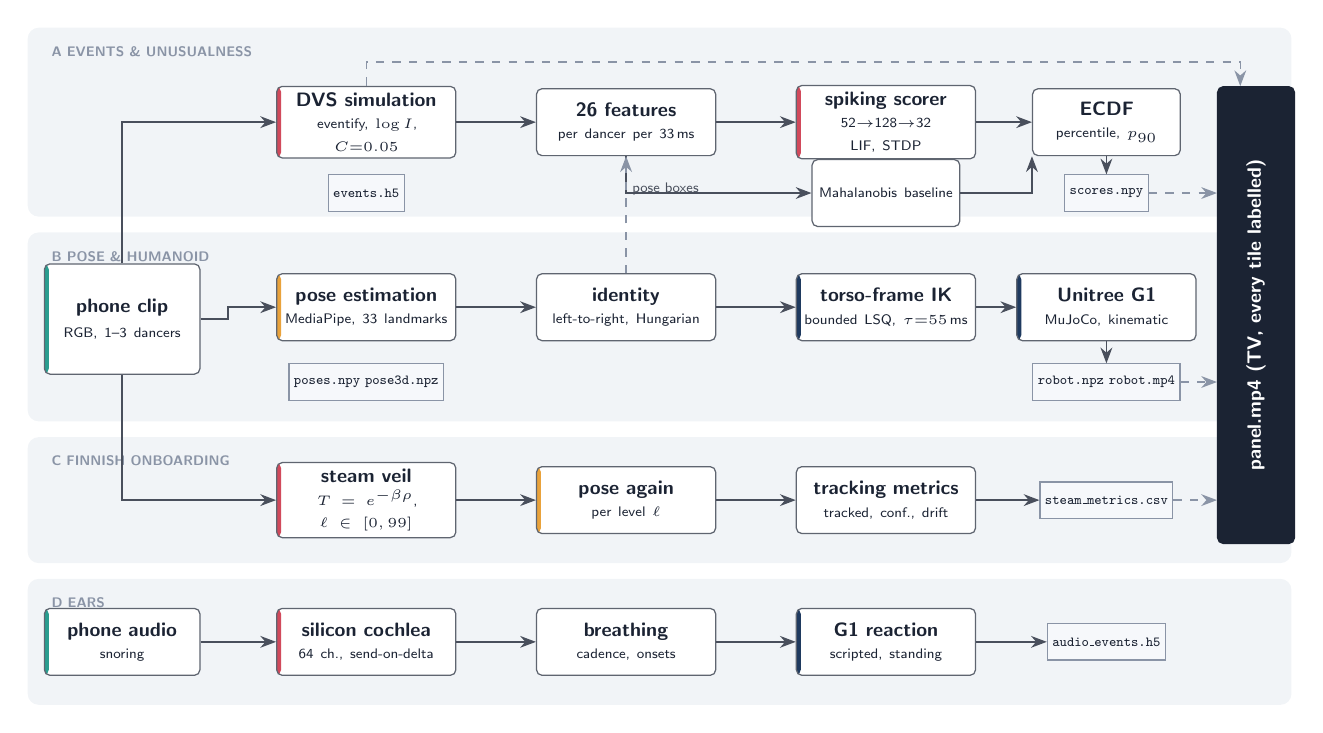
\begin{tikzpicture}[node distance=4mm]
\fill[lane] (-0.3,1.55) rectangle (15.75,-0.85);
\fill[lane] (-0.3,-1.05) rectangle (15.75,-3.45);
\fill[lane] (-0.3,-3.65) rectangle (15.75,-5.25);
\fill[lane] (-0.3,-5.45) rectangle (15.75,-7.05);
\node[lanelabel] at (-0.12,1.43) {A\,\,EVENTS \& UNUSUALNESS};
\node[lanelabel] at (-0.12,-1.17) {B\,\,POSE \& HUMANOID};
\node[lanelabel] at (-0.12,-3.77) {C\,\,FINNISH ONBOARDING};
\node[lanelabel] at (-0.12,-5.57) {D\,\,EARS};
% input
\node[real, text width=18mm, minimum height=14mm] (clip) at (0.9,-2.15) {\textbf{phone clip}\\[1pt]\tiny RGB, 1--3 dancers};
% lane A
\node[sim] (dvs) at (4.0,0.35) {\textbf{DVS simulation}\\\tiny eventify, $\log I$, $C{=}0.05$};
\node[file] (evh5) at (4.0,-0.55) {events.h5};
\node[box] (feat) at (7.3,0.35) {\textbf{26 features}\\\tiny per dancer per 33\,ms};
\node[sim] (snn) at (10.6,0.35) {\textbf{spiking scorer}\\\tiny 52$\to$128$\to$32 LIF, STDP};
\node[box, text width=17mm] (maha) at (10.6,-0.55) {\tiny Mahalanobis baseline};
\node[box, text width=17mm] (ecdf) at (13.4,0.35) {\textbf{ECDF}\\\tiny percentile, $p_{90}$};
\node[file] (scores) at (13.4,-0.55) {scores.npy};
% lane B
\node[est] (pose) at (4.0,-2.0) {\textbf{pose estimation}\\\tiny MediaPipe, 33 landmarks};
\node[file] (poses) at (4.0,-2.95) {poses.npy\,\,pose3d.npz};
\node[box] (track) at (7.3,-2.0) {\textbf{identity}\\\tiny left-to-right, Hungarian};
\node[rep] (ik) at (10.6,-2.0) {\textbf{torso-frame IK}\\\tiny bounded LSQ, $\tau{=}55$\,ms};
\node[rep] (g1) at (13.4,-2.0) {\textbf{Unitree G1}\\\tiny MuJoCo, kinematic};
\node[file] (robot) at (13.4,-2.95) {robot.npz\,\,robot.mp4};
% lane C
\node[sim] (steam) at (4.0,-4.45) {\textbf{steam veil}\\\tiny $T=e^{-\beta\rho}$, $\ell\in[0,99]$};
\node[est] (pose2) at (7.3,-4.45) {\textbf{pose again}\\\tiny per level $\ell$};
\node[box] (metrics) at (10.6,-4.45) {\textbf{tracking metrics}\\\tiny tracked, conf., drift};
\node[file] (csv) at (13.4,-4.45) {steam\_metrics.csv};
% lane D
\node[real, text width=18mm] (audio) at (0.9,-6.25) {\textbf{phone audio}\\\tiny snoring};
\node[sim] (coch) at (4.0,-6.25) {\textbf{silicon cochlea}\\\tiny 64 ch., send-on-delta};
\node[box] (breath) at (7.3,-6.25) {\textbf{breathing}\\\tiny cadence, onsets};
\node[rep] (sleep) at (10.6,-6.25) {\textbf{G1 reaction}\\\tiny scripted, standing};
\node[file] (ears) at (13.4,-6.25) {audio\_events.h5};
% viewer
\node[box, fill=ink, text=white, draw=ink, text width=8mm, minimum height=58mm, rotate=0] (tv) at (15.3,-2.1) {};
\node[font=\sffamily\scriptsize\bfseries, text=white, rotate=90] at (15.3,-2.1) {panel.mp4  (TV, every tile labelled)};
% flows
\draw[flow] (clip.north) |- (dvs.west);
\draw[flow] (clip.east) -- ++(0.35,0) |- (pose.west);
\draw[flow] (clip.south) |- (steam.west);
\draw[flow] (dvs) -- (feat); \draw[flow] (feat) -- (snn); \draw[flow] (snn) -- (ecdf);
\draw[flow] (feat.south) |- (maha.west); \draw[flow] (maha.east) -| (ecdf.south west);
\draw[flow] (ecdf) -- (scores);
\draw[flow] (pose) -- (track); \draw[flow] (track) -- (ik); \draw[flow] (ik) -- (g1); \draw[flow] (g1) -- (robot);
\draw[flowd] (track.north) -- node[note, right, pos=0.72, xshift=1pt]{pose boxes} (feat.south);
\draw[flow] (steam) -- (pose2); \draw[flow] (pose2) -- (metrics); \draw[flow] (metrics) -- (csv);
\draw[flow] (audio) -- (coch); \draw[flow] (coch) -- (breath); \draw[flow] (breath) -- (sleep); \draw[flow] (sleep) -- (ears);
\foreach \n in {scores, robot, csv} \draw[flowd] (\n.east) -- (\n.east -| tv.west);
\draw[flowd] (dvs.north) -- ++(0,0.3) -| ([xshift=-2mm]tv.north);
\end{tikzpicture}
}
  \caption[The VLMA pipeline]{\textbf{The \vlma{} pipeline.} The coloured bar on each stage gives the status of its output: \legendchip{realc}{real}, \legendchip{simc}{simulated}, \legendchip{estc}{estimated}, \legendchip{repc}{kinematic replay}. Grey boxes are deterministic transforms. Files in monospace are the contract between team members (\cref{fig:schema}). Pose boxes from lane B crop the event features in lane A when available; otherwise the scorer uses self-centring vertical strips.}
  \label{fig:pipeline}
\end{figure}

\begin{figure}[t]
  \centering
  \resizebox{\linewidth}{!}{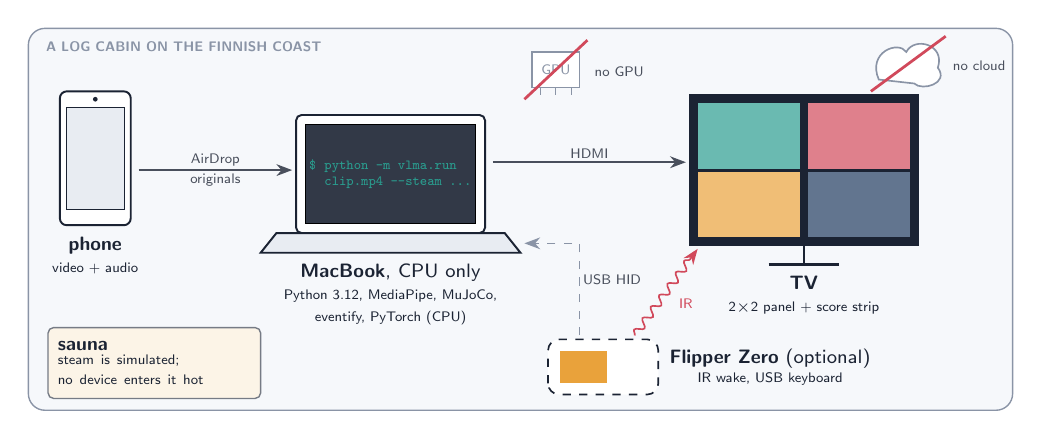
\begin{tikzpicture}
\draw[draw=slate, line width=0.5pt, rounded corners=6pt, fill=paper] (-0.4,-0.75) rectangle (12.1,4.1);
\node[font=\sffamily\tiny\bfseries, text=slate, anchor=north west] at (-0.3,4.05) {A LOG CABIN ON THE FINNISH COAST};
% phone
\draw[ink, line width=0.7pt, rounded corners=2.5pt, fill=white] (0,1.6) rectangle (0.9,3.3);
\draw[ink, fill=mist] (0.08,1.8) rectangle (0.82,3.1);
\fill[ink] (0.45,3.2) circle (0.03);
\node[base, anchor=north] at (0.45,1.55) {\textbf{phone}\\\tiny video + audio};
% macbook
\draw[ink, line width=0.7pt, rounded corners=2pt, fill=white] (3.0,1.5) rectangle (5.4,3.0);
\draw[fill=ink!90] (3.12,1.62) rectangle (5.28,2.88);
\node[font=\ttfamily\tiny, text=teal, align=left] at (4.2,2.25) {\$ python -m vlma.run\\\ \ clip.mp4 --steam ...};
\draw[ink, line width=0.7pt, fill=mist] (2.75,1.5) -- (5.65,1.5) -- (5.85,1.25) -- (2.55,1.25) -- cycle;
\node[base, anchor=north] at (4.2,1.2) {\textbf{MacBook}, CPU only\\\tiny Python 3.12, MediaPipe, MuJoCo,\\\tiny eventify, PyTorch (CPU)};
% TV
\draw[ink, line width=0.9pt, fill=ink] (8.0,1.35) rectangle (10.9,3.25);
\foreach \x/\y/\c in {8.1/2.32/teal, 9.5/2.32/coral, 8.1/1.45/amber, 9.5/1.45/navy}
  \fill[\c!70] (\x,\y) rectangle ++(1.3,0.83);
\draw[ink, line width=0.9pt] (9.45,1.35) -- (9.45,1.1) (9.0,1.1) -- (9.9,1.1);
\node[base, anchor=north] at (9.45,1.05) {\textbf{TV}\\\tiny 2$\times$2 panel + score strip};
% flipper
\draw[ink, line width=0.6pt, rounded corners=4pt, fill=white, dashed] (6.2,-0.55) rectangle (7.6,0.15);
\fill[amber] (6.35,-0.4) rectangle (6.95,0.0);
\node[base, anchor=west] at (7.65,-0.2) {\textbf{Flipper Zero} (optional)\\[-1pt]\tiny IR wake, USB keyboard};
% links
\draw[flow] (1.0,2.3) -- node[note, above]{AirDrop} node[note, below]{originals} (2.95,2.3);
\draw[flow] (5.5,2.4) -- node[note, above]{HDMI} (7.95,2.4);
\draw[irwave, ->] (7.3,0.2) -- (8.1,1.3);
\node[note, text=coral] at (7.95,0.6) {IR};
\draw[flowd] (6.6,0.2) |- node[note, right, pos=0.3]{USB HID} (5.9,1.37);
% crossed out
\begin{scope}[shift={(10.75,3.55)}]
\draw[slate, line width=0.6pt, fill=white] (-0.35,-0.1) .. controls (-0.5,0.25) and (-0.1,0.4) .. (0,0.25) .. controls (0.1,0.45) and (0.5,0.35) .. (0.4,0.05) .. controls (0.55,-0.15) and (0.2,-0.25) .. (0.1,-0.15) -- cycle;
\draw[cross] (-0.45,-0.25) -- (0.5,0.45); \node[note, anchor=west] at (0.55,0.08) {no cloud};
\end{scope}
\begin{scope}[shift={(6.3,3.55)}]
\draw[slate, line width=0.6pt, fill=white] (-0.3,-0.2) rectangle (0.3,0.25);
\foreach \x in {-0.2,0,0.2} \draw[slate] (\x,-0.2) -- (\x,-0.3);
\node[font=\sffamily\tiny, text=slate] at (0,0.02) {GPU};
\draw[cross] (-0.4,-0.35) -- (0.4,0.4); \node[note, anchor=west] at (0.45,0.0) {no GPU};
\end{scope}
% sauna
\draw[ink!60, line width=0.5pt, fill=amber!12, rounded corners=2pt] (-0.15,-0.6) rectangle (2.55,0.3);
\node[base, anchor=west, text width=25mm, align=left] at (-0.12,-0.15) {\textbf{sauna}\\[-1pt]\tiny steam is simulated;\\[-1pt]\tiny no device enters it hot};
\end{tikzpicture}
}
  \caption[Deployment: phone, laptop, TV, optional Flipper Zero]{\textbf{Deployment.} One phone, one MacBook (CPU only), one TV, and an optional Flipper Zero that can wake the TV over infrared and type the launch command as a USB keyboard~\cite{flipperdocs}, using only the TV's own remote codes and the team's own hardware. Nothing leaves the cabin: no cloud, no GPU. No device enters a hot sauna; the steam in this paper is simulated.}
  \label{fig:hardware}
\end{figure}

\begin{figure}[t]
  \centering
  \resizebox{\linewidth}{!}{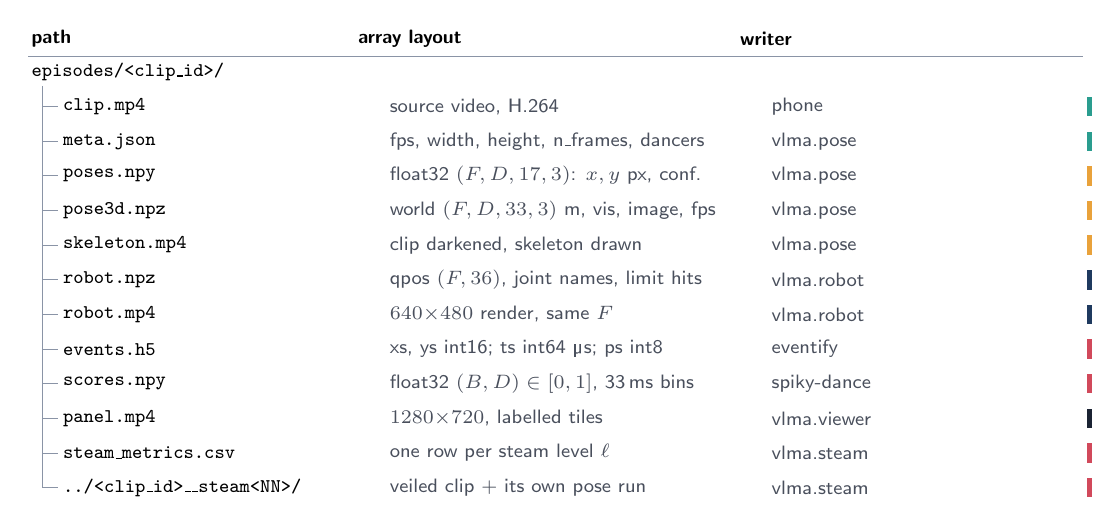
\begin{tikzpicture}[every node/.style={font=\ttfamily\scriptsize, anchor=west, inner sep=1pt}, x=1cm, y=0.44cm]
\def\row#1#2#3#4#5{%
  \node at (0,-#1) {#2};
  \node[font=\sffamily\scriptsize, text=ink!80] at (4.15,-#1) {#3};
  \node[font=\sffamily\scriptsize, text=ink!80] at (9.0,-#1) {#4};
  \fill[#5] (13.05,-#1-0.28) rectangle ++(1.6pt,0.56);
}
\node[font=\sffamily\scriptsize\bfseries] at (0,0.95) {path};
\node[font=\sffamily\scriptsize\bfseries] at (4.15,0.95) {array layout};
\node[font=\sffamily\scriptsize\bfseries] at (9.0,0.95) {writer};
\draw[slate, line width=0.4pt] (0,0.45) -- (13.4,0.45);
\node[font=\ttfamily\scriptsize\bfseries] at (0,0) {episodes/<clip\_id>/};
\draw[slate] (0.18,-0.4) -- (0.18,-12);
\foreach \i in {1,...,12} \draw[slate] (0.18,-\i) -- (0.38,-\i);
\begin{scope}[xshift=4mm]
\row{1}{clip.mp4}{source video, H.264}{phone}{realc}
\row{2}{meta.json}{fps, width, height, n\_frames, dancers}{vlma.pose}{realc}
\row{3}{poses.npy}{float32 $(F, D, 17, 3)$: $x, y$ px, conf.}{vlma.pose}{estc}
\row{4}{pose3d.npz}{world $(F,D,33,3)$ m, vis, image, fps}{vlma.pose}{estc}
\row{5}{skeleton.mp4}{clip darkened, skeleton drawn}{vlma.pose}{estc}
\row{6}{robot.npz}{qpos $(F, 36)$, joint names, limit hits}{vlma.robot}{repc}
\row{7}{robot.mp4}{$640{\times}480$ render, same $F$}{vlma.robot}{repc}
\row{8}{events.h5}{xs, ys int16; ts int64 \textmu s; ps int8}{eventify}{simc}
\row{9}{scores.npy}{float32 $(B, D)\in[0,1]$, 33\,ms bins}{spiky-dance}{simc}
\row{10}{panel.mp4}{$1280{\times}720$, labelled tiles}{vlma.viewer}{ink}
\row{11}{steam\_metrics.csv}{one row per steam level $\ell$}{vlma.steam}{simc}
\row{12}{../<clip\_id>\_\_steam<NN>/}{veiled clip + its own pose run}{vlma.steam}{simc}
\end{scope}
\end{tikzpicture}
}
  \caption[The episode contract]{\textbf{The episode contract.} One folder per clip; $F$ frames, $D\le3$ dancers, $B$ score bins of 33\,ms. Dancer 0 is the leftmost. A missing joint has confidence 0; a missing stream is shown as ``not available yet'', never filled. The bar gives each file's status as in \cref{fig:pipeline}.}
  \label{fig:schema}
\end{figure}

\begin{algorithm}[t]
\caption{\textsc{VLMA-Run}: one command, clip in, episode and TV video out}
\label{alg:run}
\small
\begin{algorithmic}[1]
\Require clip $V$; optional event command $\mathcal{E}$, score command $\mathcal{S}$, steam levels $\mathcal{L}$
\State $E \gets$ \file{episodes/}$\,\mathrm{stem}(V)$ \Comment{episode folder}
\State $(P_{2D}, P_{3D}, \mathrm{vis}) \gets \textsc{Pose}(V)$ \Comment{MediaPipe, $\le3$ dancers, left-to-right identity}
\State $q_{1:F} \gets \textsc{Retarget}(P_{3D}, \mathrm{vis})$; render G1 \Comment{\cref{eq:ik,eq:smooth}}
\If{$\mathcal{E}$} run $\mathcal{E}(V, E)$ \Comment{simulated events, \file{events.h5}} \EndIf
\If{$\mathcal{S}$} run $\mathcal{S}(V, E)$ \Comment{scores in $[0,1]$, \file{scores.npy}} \EndIf
\State \textsc{Viewer}$(E)$ \Comment{labelled $2{\times}2$ panel, missing tiles say so}
\For{$\ell \in \mathcal{L}$} \Comment{Finnish onboarding}
  \State $V_\ell \gets \textsc{Steam}(V, \ell, \text{seed}=0)$ \Comment{\cref{eq:steam}, lossless}
  \State $m_\ell \gets \textsc{Pose}(V_\ell)$ with the clean dancer count; drift vs.\ clean \Comment{\cref{eq:drift}}
\EndFor
\State write \file{steam\_metrics.csv}, stage timings
\end{algorithmic}
\end{algorithm}

\begin{table}[t]
\centering
\caption{\textbf{What is real and what is simulated.} The same labels appear on every tile of the TV output and in every file name and caption in this paper.}
\label{tab:realsim}
\small
\begin{tabularx}{\linewidth}{@{}l l X@{}}
\toprule
Stream & Status & Source and caveat \\
\midrule
Phone video & \realtag & Recorded clip; other people's video stays out of the repository unless they agreed. \\
Snoring audio & \realtag & Real recording; only derived, simulated events are stored. \\
Event-camera stream & \simtag & eventify frame-difference model on the video. We have no event camera. \\
Pose skeleton & \esttag & MediaPipe Pose Landmarker (full). Not ground truth. \\
Humanoid & \reptag & Kinematic replay with joint limits. No physics balance, no controller, no learning. \\
Physics G1 & \simtag & RL policy in simulated rigid-body physics, trained on the replay. Not run on a real robot. \\
Unusualness score & \simtag{} input & Network output on simulated events; trained on 21 clean real clips, including our five takes. \\
Steam & \simtag & Analytic veil; not fitted to real steam. The tracking curve under it is measured. \\
Cochlea events & \simtag & Software filterbank and comparators; not a chip model, not a medical device. \\
\bottomrule
\end{tabularx}
\end{table}

\section{Method}
\label{sec:method}

\subsection{Simulated event camera}
\label{sec:dvs}

An idealised DVS pixel fires when its log intensity changes by a contrast threshold $C$~\cite{lichtsteiner2008dvs,gallego2022survey}. With grey level $I_k(\mathbf{x}) \in [0,255]$ of frame $k$, resized to the sensor resolution ($\EvW{\times}\EvH$), and offset $\varepsilon=1$, eventify computes
\begin{equation}
  \Delta L_k(\mathbf{x}) = \log\!\big(I_k(\mathbf{x})+\varepsilon\big) - \log\!\big(I_{k-1}(\mathbf{x})+\varepsilon\big), \qquad
  N_k(\mathbf{x}) = \left\lfloor \frac{|\Delta L_k(\mathbf{x})|}{C} \right\rfloor ,
  \label{eq:dvs}
\end{equation}
and emits $N_k(\mathbf{x})$ events of polarity $p=\mathbb{1}[\Delta L_k>0]$ at times $t_{k-1} + \frac{j}{N_k+1}(t_k - t_{k-1})$, $j=1,\dots,N_k$, so that events at one pixel are strictly ordered. We use $C=0.05$. Optional interpolated sub-frames (\texttt{interp}$=3$ in the scorer's training) reduce the temporal quantisation. The model has no noise, no refractory period and no bandwidth limit, unlike v2e~\cite{hu2021v2e}; the events are therefore cleaner than a real sensor would give.

\subsection{Pose estimation, COCO mapping and identity}
\label{sec:pose}

MediaPipe Pose Landmarker (full) runs in video mode with up to three poses per frame and returns 33 image landmarks, 33 metric world landmarks and per-landmark visibility. We export COCO-17 by the index map
\begin{equation}
  \pi = (0, 2, 5, 7, 8, 11, 12, 13, 14, 15, 16, 23, 24, 25, 26, 27, 28),
  \label{eq:coco}
\end{equation}
i.e.\ nose, eyes, ears, shoulders, elbows, wrists, hips, knees and ankles, scaled to pixels of the original video, with visibility as confidence. Identity is anchored at the first frame with $D$ detections by sorting hip centres left to right, then propagated forwards and backwards by Hungarian assignment~\cite{kuhn1955hungarian} on hip-centre distance,
\begin{equation}
  \sigma_t^\star = \arg\min_{\sigma\in\mathfrak{S}} \sum_{d} \big\|\mathbf{h}_{t,\sigma(d)} - \mathbf{h}_{t\mp1,d}\big\|_2, \qquad \mathbf{h} = \tfrac12(\mathbf{k}_{\text{l.hip}}+\mathbf{k}_{\text{r.hip}}),
  \label{eq:hungarian}
\end{equation}
over one-to-one matchings $\sigma$ of detections to dancer slots; unassigned detections fill free slots in left-to-right order. The dancer count $D$ is the largest $n\le3$ observed in at least 10\% of frames.

\subsection{Torso-frame retargeting onto the G1}
\label{sec:ik}

No source axis is hard-coded. For world landmarks $\mathbf{p}_i$ (shoulders 11, 12; hips 23, 24) we build a per-frame torso basis
\begin{equation}
  \mathbf{l} = \nrm(\mathbf{p}_{11}-\mathbf{p}_{12}), \quad
  \bar{\mathbf{u}} = \tfrac12(\mathbf{p}_{11}+\mathbf{p}_{12}-\mathbf{p}_{23}-\mathbf{p}_{24}), \quad
  \mathbf{u} = \nrm\big(\bar{\mathbf{u}} - (\bar{\mathbf{u}}^{\!\top}\mathbf{l})\,\mathbf{l}\big), \quad
  \mathbf{f} = \mathbf{l}\times\mathbf{u},
  \label{eq:torso}
\end{equation}
and $R=[\mathbf{f}\;\mathbf{l}\;\mathbf{u}]$. For each arm with shoulder, elbow and wrist $(\mathbf{s},\mathbf{e},\mathbf{w})$ the targets are the bone directions in the torso frame, $\mathbf{d}_1 = R^{\!\top}\nrm(\mathbf{e}-\mathbf{s})$ and $\mathbf{d}_2 = R^{\!\top}\nrm(\mathbf{w}-\mathbf{e})$. With $q\in\R^4$ the shoulder pitch, roll, yaw and elbow angles and $\hat{\mathbf{u}}_1(q),\hat{\mathbf{u}}_2(q)$ the upper-arm and forearm directions of the G1 from MuJoCo forward kinematics at the standing keyframe, we solve
\begin{equation}
  q^\star_t = \arg\min_{q_{\min}\le q\le q_{\max}} \;\big\| \hat{\mathbf{u}}_1(q)-\mathbf{d}_1 \big\|^2 + \big\| \hat{\mathbf{u}}_2(q)-\mathbf{d}_2 \big\|^2
  \label{eq:ik}
\end{equation}
by trust-region reflective least squares~\cite{branch1999trf} warm-started at $q_{t-1}$, at most 35 evaluations, finite-difference step $10^{-4}$. Frames whose torso or arm landmarks have visibility below 0.3 hold the previous pose. A first-order filter with time constant $\tau=55$\,ms keeps the swing and removes landmark jitter:
\begin{equation}
  q_t = q_{t-1} + \alpha\,(q^\star_t - q_{t-1}), \qquad \alpha = 1 - e^{-1/(f_s \tau)},
  \label{eq:smooth}
\end{equation}
with $f_s$ the video frame rate. Base and legs stay at the standing keyframe; palm orientation is not recovered. Saturated joints are counted before filtering as limit hits.

\subsection{Event features}
\label{sec:features}

Events are binned into 33\,ms windows. For dancer $d$ in bin $k$, inside the dancer's box (pose keypoints padded by 15\% per side, or a self-centring vertical strip that follows a 5\,s running median of event positions), with $n$ events of which $n_{+}$ are ON at box-normalised positions $(\tilde x_j,\tilde y_j)$:
\begin{equation}
  \underbrace{\frac{r}{1+r}}_{\text{rate},\; r = n/\bar n_{10\,\mathrm{s}}}, \quad
  \underbrace{\frac{n_+ - n_-}{n}}_{\text{polarity}}, \quad
  \underbrace{\tfrac1n\textstyle\sum_j \tilde x_j,\; \tfrac1n\sum_j \tilde y_j}_{\text{centroid}}, \quad
  \underbrace{\big(\tfrac{n_{ab}}{n}\big)_{a,b\in\{1,2,3\}}}_{3\times3 \text{ grid}},
  \label{eq:features}
\end{equation}
13 values $\mathbf{x}_k\in\R^{13}$, where $\bar n_{10\,\mathrm{s}}$ is the dancer's own running mean over 300 bins, so 0.5 is the dancer's normal level. The feature vector is $[\mathbf{x}_k;\, \mathbf{x}_k-\mathbf{x}_{k-1}] \in\R^{26}$. Empty bins give rate 0, polarity 0, centroid 0.5 and an empty grid, never NaN.

\subsection{Spiking unusualness scorer}
\label{sec:scorer}

The scorer is adapted from Mr.\ Spiky, a team member's earlier spiking network for scoring source code. Kept: the layer sizes, STDP rule and settings, ZCA whitening, per-neuron baselines and percentile calibration. Changed: adaptive thresholds, top-$k$ inhibition, weight normalisation and on/off encoding.

\paragraph{Whitening and on/off encoding.} Features are mapped to $[0,1]$ and ZCA-whitened~\cite{kessy2018whitening}, $\mathbf{y} = c\,\Sigma^{-1/2}(\tilde{\mathbf{x}}-\bm\mu)$ with eigenvalues floored at $10^{-3}$ and $c$ chosen so that the 99th percentile of $|y|$ is 0.5. Each whitened value gives two non-negative inputs,
\begin{equation}
  \mathbf{s} = \clip\!\big(g\,[\relu(\mathbf{y});\, \relu(-\mathbf{y})],\,0,1\big)\in[0,1]^{52}, \qquad g = 2,
  \label{eq:onoff}
\end{equation}
so a normal bin gives near-zero input and a deviation in either direction raises one input. The original encoding, $\clip(\mathbf{y}+0.5,0,1)$, gives every input a constant 0.5 and lets a below-mean value \emph{lower} the current; it cannot see a freeze (\cref{sec:exp-scorer}).

\paragraph{LIF dynamics with top-$k$ inhibition.} Two layers, $52\to128\to32$, no bias, non-negative weights. For layer $\ell$ with input $\mathbf{z}^{\ell-1}_t$:
\begin{equation}
  \mathbf{v}_t = \beta\,\mathbf{m}_{t-1} + W\mathbf{z}^{\ell-1}_t, \qquad
  z_{t,i} = \mathbb{1}\big[v_{t,i} > \vartheta_i\big]\cdot\mathbb{1}\big[v_{t,i}-\vartheta_i \ge \kappa_t\big],
  \label{eq:lif}
\end{equation}
with $\beta=0.9$, $\kappa_t$ the $k$-th largest excess $v_{t,i}-\vartheta_i$ in the layer, $k=\mathrm{round}(0.15N)$. Winners reset by subtraction, $m_{t,i}=v_{t,i}-\vartheta_i$; suppressed neurons above threshold are clamped to it, $m_{t,i}=\min(v_{t,i},\vartheta_i)$.

\paragraph{Adaptive thresholds.} Each neuron has threshold $\vartheta_i = \max(1+\theta_i,\, 0.05)$; during training
\begin{equation}
  \theta_i \leftarrow \theta_i + \eta\,(z_{t,i} - \rho^\ast), \qquad \eta = 0.02,\; \rho^\ast = 0.10,
  \label{eq:homeo}
\end{equation}
which drives every neuron toward firing in 10\% of steps. For scoring, $\theta$ is frozen.

\paragraph{STDP.} Training uses rate-coded binary spikes (25 steps per bin). With exponentially decaying traces $\mathbf{x}^{\mathrm{pre}}_t = \lambda\mathbf{x}^{\mathrm{pre}}_{t-1}+\mathbf{z}^{\mathrm{pre}}_t$ and likewise $\mathbf{x}^{\mathrm{post}}$, $\lambda=e^{-1/20}$, the pair-based rule with multiplicative depression~\cite{bi1998stdp,diehl2015unsupervised} is
\begin{equation}
  \Delta W = \sum_t A_{+}\, \mathbf{z}^{\mathrm{post}}_t \big(\mathbf{x}^{\mathrm{pre}}_t\big)^{\!\top} - A_{-}\, \big(\mathbf{x}^{\mathrm{post}}_t \big(\mathbf{z}^{\mathrm{pre}}_t\big)^{\!\top}\big)\odot W,
  \qquad A_{+}=0.005,\; A_{-}=0.020,
  \label{eq:stdp}
\end{equation}
followed by $W\leftarrow\clip\big((1-10^{-3})W+\Delta W,\,0,1\big)$ and row normalisation $\sum_j W_{ij} = 0.25\,n_{\mathrm{in}}$. Six epochs.

\paragraph{Raw score and percentile calibration.} In scoring mode, whitened inputs enter as graded currents, one step per bin. With membrane potentials $v$ shifted by each neuron's threshold offset and per-neuron baseline firing rates $b_i$ on the clean corpus,
\begin{equation}
  a_{t,i} = \frac{\big[\sigma(4(v_{t,i}-\vartheta_i)) - b_i\big]_+}{1-b_i}, \qquad
  r_t = \tfrac12\,\overline{a}^{\,\mathrm{hid}}_t + \tfrac12\,\overline{a}^{\,\mathrm{out}}_t,
  \qquad
  s_t = \hat F_{\mathrm{clean}}(r_t) = \frac{\#\{\,r' \in \mathcal{R}_{\mathrm{clean}} : r'\le r_t\,\}}{|\mathcal{R}_{\mathrm{clean}}|}.
  \label{eq:ecdf}
\end{equation}
A score is a percentile against clean dancing: 0.5 is the clean median and the threshold $s>0.90$ marks the top 10\%. A normal held-out clip should therefore give a mean near 0.5 and about 10\% of bins above threshold.

\paragraph{Baseline.} The Mahalanobis scorer~\cite{mahalanobis1936} fits $\bm\mu,\Sigma$ on clean bins and scores $r=\sqrt{(\mathbf{x}-\bm\mu)^{\!\top}(\Sigma+10^{-3}I)^{-1}(\mathbf{x}-\bm\mu)}$, calibrated by the same ECDF. It is stateless across bins.

\paragraph{Sync score.} For $D\ge2$ dancers a training-free score compares each dancer with the median of the others, feature by feature, over a rolling window $\mathcal{W}_t$ of 2\,s:
\begin{equation}
  \mathrm{sync}_{t,d} = 1 - \frac{1}{13}\sum_{f=1}^{13} \operatorname{corr}_{\mathcal{W}_t}\!\Big(x^{(f)}_{\cdot,d},\; \operatorname*{median}_{d'\neq d} x^{(f)}_{\cdot,d'}\Big) \in [0,2],
  \label{eq:sync}
\end{equation}
so 0 is in step, 1 unrelated and 2 opposite; a feature that is constant for both series counts as correlation 1, for one of them as 0.

\subsection{Finnish onboarding: a steam veil}
\label{sec:steam}

Koschmieder's law~\cite{koschmieder1924,narasimhan2002vision} models an image through a scattering medium as $I = J\,T + A\,(1-T)$ with transmittance $T=e^{-\beta d}$, extinction $\beta$ and airlight $A$. We replace depth by a drifting column density. With $\mathcal{N}_i$ uniform noise fields of $8^2$, $16^2$ and $32^2$ cells (seed 0), bicubically upsampled and scrolled upwards at $0.35+0.17i$ cells per second, and a rising puff $G$ on a 9\,s cycle,
\begin{equation}
  \rho(\mathbf{x},t) = 0.35 + 0.85\,\Big[\textstyle\sum_{i=0}^{2} 2^{-i}\,\mathcal{N}_i(\mathbf{x},t)\Big]_+ + 0.8\sin^2(\pi\phi_t)\,G(\mathbf{x};\mathbf{c}_t,r_t), \qquad
  \beta = 5\,\ell/100,
  \label{eq:density}
\end{equation}
for steam level $\ell\in[0,99]$. The veiled frame adds forward scattering as a Gaussian blur of width $\sigma=0.3+0.35\beta$ px weighted by the scattered fraction, then the airlight $A=(235,233,228)$:
\begin{equation}
  T = e^{-\beta\rho}, \qquad
  S = T\,J + (1-T)\,(G_\sigma * J), \qquad
  I = T\,S + (1-T)\,A .
  \label{eq:steam}
\end{equation}
Level 0 is bit-exact: frames are written losslessly (\texttt{libx264rgb}, CRF 0). For each level we re-run pose with the clean dancer count and measure the tracked fraction, mean keypoint confidence, and confidence-weighted drift against the clean run,
\begin{equation}
  \delta = \frac{\sum_{t,j} w_{tj}\,\|\mathbf{k}^{\ell}_{tj} - \mathbf{k}^{0}_{tj}\|}{\sum_{t,j} w_{tj}}, \qquad w_{tj} = \min(c^{\ell}_{tj}, c^{0}_{tj}).
  \label{eq:drift}
\end{equation}

\subsection{Robot ears: a simulated silicon cochlea}
\label{sec:ears}

Audio is decoded to 16\,kHz mono in memory and never stored. \SnoreChannels{} channels with centres $f_c$ log-spaced from 50\,Hz to 4\,kHz each apply a second-order Butterworth band-pass $H_c$ of $\pm\frac16$ octave, half-wave rectification and a 200\,Hz low-pass $H_{\mathrm{lp}}$, sampled at 4\,kHz:
\begin{equation}
  f_c = 50\cdot 80^{\,c/(N_c-1)}\ \mathrm{Hz},\qquad \big[f_c\,2^{-1/6},\; f_c\,2^{1/6}\big], \qquad
  e_c = H_{\mathrm{lp}} * \big[H_c * a\big]_+ ,
  \label{eq:filterbank}
\end{equation}
with $a$ the audio and $N_c=\SnoreChannels$. Each envelope $e_c$ is log-compressed, $L_c=\log(1+e_c/\phi_c)$ with $\phi_c = 0.005\cdot p_{90}(e_c)$, and drives a send-on-delta comparator as in a DVS pixel:
\begin{equation}
  |L_c(t) - L^{\mathrm{ref}}_c| \ge \theta \;\Rightarrow\; \text{event}(c,t,\operatorname{sign}),\quad L^{\mathrm{ref}}_c \leftarrow L^{\mathrm{ref}}_c \pm \theta,
  \label{eq:cochlea}
\end{equation}
with $\theta=\SnoreTheta$ and a 1\,ms refractory period. Breathing is read from the 50--1000\,Hz RMS envelope $u$ at 20\,Hz with 200\,ms Gaussian smoothing. With $\tilde u = u-\bar u$ and normalised autocorrelation $R(\tau)$,
\begin{equation}
  R(\tau) = \frac{\sum_n \tilde u_n\,\tilde u_{n+\tau}}{\sum_n \tilde u_n^2}, \qquad
  \tau^\star = \operatorname*{arg\,max}_{\tau\in[1.5,\,8]\,\mathrm{s},\;\tau\ \text{a local peak}} R(\tau), \qquad
  \text{breaths/min} = \frac{60}{\tau^\star},
  \label{eq:cadence}
\end{equation}
accepted when $R(\tau^\star)\ge0.1$. Snore onsets are envelope peaks with prominence at least 20\% of the 10th-to-95th percentile range, timed at the rising quarter-prominence crossing; a gap longer than $\max(10\,\mathrm{s},\,2.5\times$ the median gap$)$ is flagged as a pause. The G1's reaction to the sound is scripted, standing, and clamped to joint limits.

\subsection{From replay to physics: whole-body motion tracking}
\label{sec:physics}

The kinematic replay cannot fall, so it proves nothing about a real robot. We therefore train a policy that drives the G1's 29 joints in rigid-body physics to follow the replay, in the style of DeepMimic~\cite{peng2018deepmimic}, with the open motion-tracking task of mjlab on MuJoCo Warp~\cite{todorov2012mujoco}. The reference $\hat q_{1:F}$ of \cref{eq:smooth} is resampled to 50\,Hz; forward kinematics gives reference body positions $\hat{\mathbf{p}}_b$, orientations $\hat{\mathbf{R}}_b$ and velocities $\hat{\mathbf{v}}_b,\hat{\boldsymbol\omega}_b$ for each tracked body $b$. With $\mathbf{p}_b,\mathbf{R}_b,\mathbf{v}_b,\boldsymbol\omega_b$ the simulated robot's, and an anchor body $a$ (the torso), the reward is a weighted sum of Gaussian kernels on tracking errors minus regularisers,
\begin{equation}
  r_t = \sum_{k} w_k \exp\!\Big(-\frac{e_k(t)}{\sigma_k^2}\Big) \;-\; 0.1\,\|\mathbf{a}_t-\mathbf{a}_{t-1}\|^2 \;-\; 10\,c^{\mathrm{lim}}_t \;-\; 10\,c^{\mathrm{coll}}_t,
  \label{eq:track-reward}
\end{equation}
\begin{equation}
  e_{\mathrm{pos}} = \tfrac{1}{|\mathcal{B}|}\textstyle\sum_{b}\|\hat{\mathbf{p}}_b-\mathbf{p}_b\|^2,\quad
  e_{\mathrm{ori}} = \tfrac{1}{|\mathcal{B}|}\textstyle\sum_{b}\angle\big(\hat{\mathbf{R}}_b,\mathbf{R}_b\big)^2,\quad
  e_{\mathrm{vel}} = \tfrac{1}{|\mathcal{B}|}\textstyle\sum_{b}\|\hat{\mathbf{v}}_b-\mathbf{v}_b\|^2,\quad
  e_{\omega} = \tfrac{1}{|\mathcal{B}|}\textstyle\sum_{b}\|\hat{\boldsymbol\omega}_b-\boldsymbol\omega_b\|^2,
  \label{eq:track-errors}
\end{equation}
plus the same position and orientation errors for the anchor alone. Weights and widths are those of the task: $(w,\sigma)=(0.5,0.3)$ and $(0.5,0.4)$ for anchor position and orientation, $(1,0.3)$, $(1,0.4)$, $(1,1.0)$ and $(1,3.14)$ for body position, orientation, linear and angular velocity. $c^{\mathrm{lim}}$ penalises joint-limit violations and $c^{\mathrm{coll}}$ self-collision forces above 10\,N. An episode ends when the anchor height deviates from the reference by more than 0.25\,m. The policy $\pi_\theta(\mathbf{a}_t\mid\mathbf{o}_t)$ outputs joint position targets for PD control and is trained with PPO~\cite{schulman2017ppo},
\begin{equation}
  \mathcal{L}(\theta) = \mathbb{E}_t\Big[\min\big(\rho_t(\theta)\hat A_t,\;\clip(\rho_t(\theta),1-\epsilon,1+\epsilon)\hat A_t\big)\Big], \qquad
  \rho_t = \frac{\pi_\theta(\mathbf{a}_t\mid\mathbf{o}_t)}{\pi_{\theta_{\mathrm{old}}}(\mathbf{a}_t\mid\mathbf{o}_t)},
  \label{eq:ppo}
\end{equation}
with generalised advantage estimates~\cite{schulman2016gae} $\hat A_t=\sum_{l\ge0}(\gamma\lambda)^l\delta_{t+l}$, $\delta_t=r_t+\gamma V(\mathbf{o}_{t+1})-V(\mathbf{o}_t)$, $\epsilon=0.2$, $\gamma=0.99$, $\lambda=0.95$, learning rate $10^{-3}$ and 5 epochs per update, over \PhysEnvs{} parallel environments on one \PhysGPU{} GPU.

\section{Experiments}
\label{sec:exp}

\paragraph{Setup.} Everything runs on one MacBook CPU with Python 3.12, with seeded randomness. The data are five macarena takes of one team member filmed in the cabin today (\ClipW{}$\times$\ClipH{}, \ClipFps\,fps, \TakeDSec{} to \TakeASec\,s) and one public macarena clip of another dancer (\SoloSeconds\,s, \SoloW{}$\times$\SoloH{}). The public clip is shown here only as numbers, not frames. The scorer's default model was trained by its author on 21 clean 25\,s clips, 16 cut from public videos of other dancers and our five cabin takes. The public test video and our takes are therefore in its training set; held-out numbers are the author's and are marked as such. All scores use the dancer regions the model was trained with (vertical strips). Take 3 has the largest robot arm motion (summed range of the eight arm joints \TakeCArmRange\,rad, against \TakeEArmRange{} to \TakeAArmRange{} for the others) and is used for the figures.

\subsection{Simulated event stream}
\label{sec:exp-events}

On take 3 eventify produces \EvCount{} simulated events at $\EvW{\times}\EvH$, \EvRate{}k events per second (\EvPerPixelSec{} per pixel per second), \EvOnFrac\% ON (\cref{fig:events}); the five takes range from \TakeAEvRate{}k to \TakeDEvRate{}k events per second. Events concentrate on the moving arms and the silhouette edges, as \cref{eq:dvs} predicts; the static room produces none because the simulator has no noise model.

\begin{figure}[tbp]
  \centering
  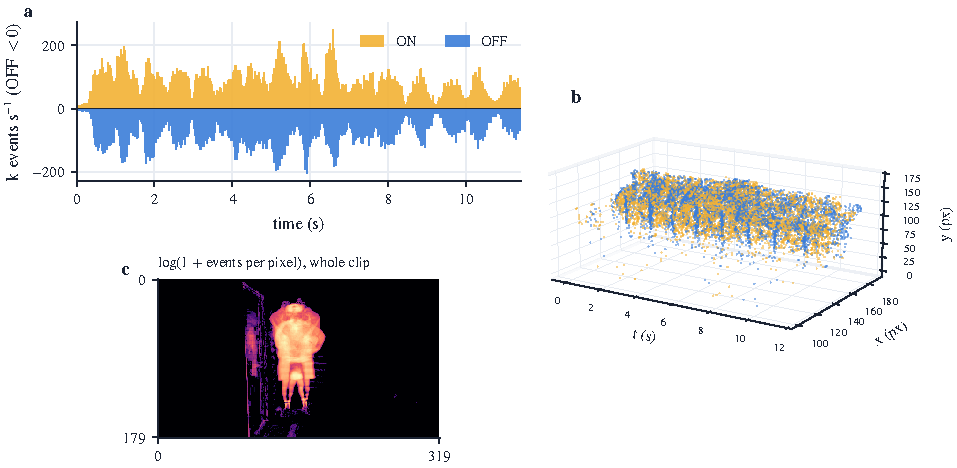
\includegraphics[width=\linewidth]{figures/out/events.pdf}
  \caption[Simulated event stream statistics]{\textbf{Simulated event stream} of take 3 (simulated from video, not sensor data). (a) ON and OFF event rates in 33\,ms bins, the scorer's bin width. (b) Space-time view of a random subsample of events. (c) Total events per pixel, log scale.}
  \label{fig:events}
\end{figure}

\subsection{Kinematic replay}
\label{sec:exp-robot}

\Cref{fig:robot} shows the eight arm joint trajectories retargeted from take 3. The macarena's structure is visible in the joints: the alternating single-arm moves of the first half give staggered left and right shoulder pitch, the hands behind the head drive both elbows to large flexion, and the hands on hips hold a steady pose at the end. At \ClipFps\,fps the filter gain of \cref{eq:smooth} is $\alpha=\SmoothAlpha$, so the replay follows within about one frame. Over \RobotFrames{} frames the solver saturated a joint limit \RobotLimitHits{} times. Palm orientation is not recovered, so the palm flip is not performed. Retargeting costs a fifth of pose estimation (\cref{tab:runtime}).

\begin{figure}[tbp]
  \centering
  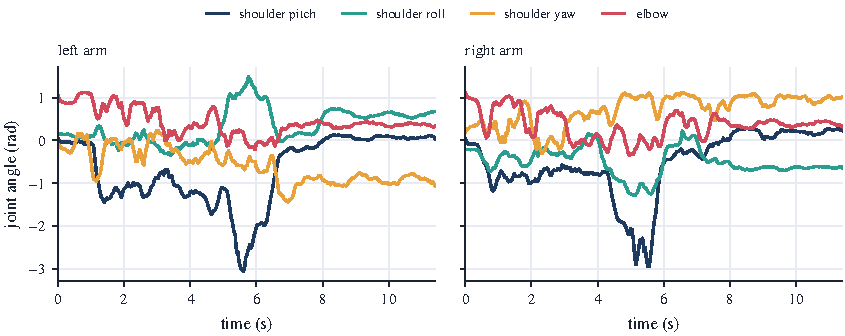
\includegraphics[width=\linewidth]{figures/out/robot_joints.pdf}
  \caption[G1 arm joint trajectories]{\textbf{G1 arm joints} from \cref{eq:ik,eq:smooth} on cabin take 3. This is a kinematic replay of estimated pose; no torques, contacts or balance are simulated.}
  \label{fig:robot}
\end{figure}

\subsection{Finnish onboarding}
\label{sec:exp-steam}

\Cref{fig:steam} and \cref{tab:steam} give the tracker's response on the public macarena clip; \cref{fig:strip} shows the same veil on our own take. Tracking is unaffected up to level 20 (\DetSTwenty\% of frames, $\bar T=\TransSTwenty$), although keypoints already drift by \DriftSTwenty\,px. It degrades at level 30 (\DetSThirty\%, $\bar T=\TransSThirty$), halves at level 40 (\DetSForty\%, confidence \ConfSForty) and is gone at level 60 (\DetSSixty\%, $\bar T=\TransSSixty$). Measured transmittance follows $e^{-\beta\bar\rho}$ with effective column density $\bar\rho=\SteamRho$ (\cref{fig:steam}b). The unusualness score reacts earlier than the tracker (the clean clip is a training clip, so the rise is relative): its mean rises from \UnuSZero{} on the clean clip to \UnuSTen{} at level 10 and \UnuSTwenty{} at level 20, where tracking is still intact. Past level 20 the score falls back slightly, to \UnuSSixty{} at level 60, because a thick veil removes the motion events it reacts to. On our own take 3 (right columns of \cref{tab:steam}) the tracker breaks one level earlier: \DetCTwenty\% of frames at level 20, \DetCThirty\% at level 30 and \DetCSixty\% at level 60. The scorer again moves first, from \UnuCZero{} clean to \UnuCTen{} at level 10 and \UnuCTwenty{} at level 20.

\begin{figure}[tbp]
  \centering
  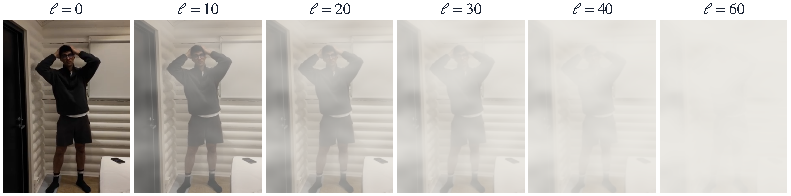
\includegraphics[width=\linewidth]{figures/out/steam_strip.pdf}
  \vspace{2pt}
  \caption[One frame of our take under rising simulated steam]{\textbf{Cabin take 3 under simulated steam}, levels 0 to 60 (\cref{eq:steam}, seed 0), at the hands-behind-head move. The veil is simulated; the measured tracking numbers in \cref{tab:steam} are for the public clip.}
  \label{fig:strip}
\end{figure}

\begin{figure}[tbp]
  \centering
  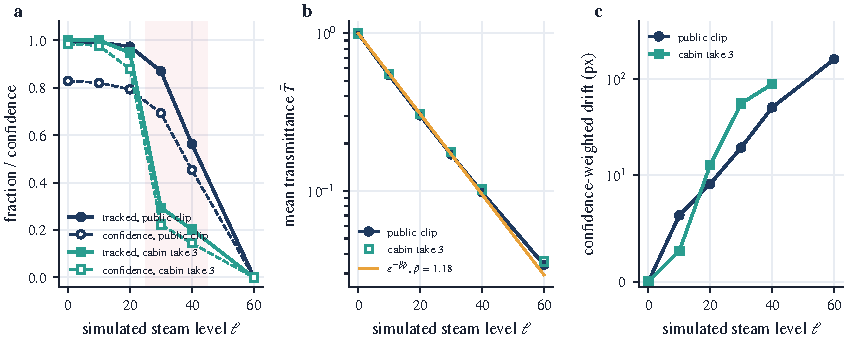
\includegraphics[width=\linewidth]{figures/out/steam_curve.pdf}
  \caption[Tracking against simulated steam]{\textbf{Tracking against simulated steam}, public macarena clip (not our footage; numbers only). (a) Fraction of frames with the dancer tracked, and mean keypoint confidence. (b) Measured mean transmittance with the fitted $e^{-\beta\bar\rho}$. (c) Confidence-weighted keypoint drift from the clean run (\cref{eq:drift}), symmetric log scale.}
  \label{fig:steam}
\end{figure}

\begin{table}[tbp]
\centering
\caption{\textbf{Steam sweep} (\file{steam\_metrics.csv}). Left: the public macarena clip. Right: our cabin take 3. Transmittance is a property of the simulated veil; tracking, confidence and drift are measured outputs of the pose model; unusualness is the mean spiking score.}
\label{tab:steam}
\small
\setlength{\tabcolsep}{4.5pt}
\begin{tabular}{@{}r c r c r c c r c@{}}
\toprule
& \multicolumn{5}{c}{Public clip} & & \multicolumn{2}{c@{}}{Cabin take 3} \\
\cmidrule(lr){2-6}\cmidrule(l){8-9}
Level $\ell$ & Mean $\bar T$ & Tracked (\%) & Confidence & Drift (px) & Unusual. & & Tracked (\%) & Unusual. \\
\midrule
0  & \TransSZero   & \DetSZero   & \ConfSZero   & \DriftSZero & \UnuSZero & & \DetCZero & \UnuCZero \\
10 & \TransSTen    & \DetSTen    & \ConfSTen    & \DriftSTen & \UnuSTen & & \DetCTen & \UnuCTen \\
20 & \TransSTwenty & \DetSTwenty & \ConfSTwenty & \DriftSTwenty & \UnuSTwenty & & \DetCTwenty & \UnuCTwenty \\
\rowcolor{coral!8} 30 & \TransSThirty & \DetSThirty & \ConfSThirty & \DriftSThirty & \UnuSThirty & & \DetCThirty & \UnuCThirty \\
\rowcolor{coral!8} 40 & \TransSForty  & \DetSForty  & \ConfSForty  & \DriftSForty & \UnuSForty & & \DetCForty & \UnuCForty \\
60 & \TransSSixty  & \DetSSixty  & \ConfSSixty  & \DriftSSixty & \UnuSSixty & & \DetCSixty & \UnuCSixty \\
\bottomrule
\end{tabular}
\end{table}

\begin{takeaway}
\textbf{Result.} Our robots are not ready for Finland. Pose tracking survives a veil that removes \LossSTwenty\% of the light and fails between \LossSThirty\% and \LossSForty\% loss. A sauna at full l\"oyly is outside the operating envelope of an off-the-shelf pose model.
\end{takeaway}

\subsection{Unusualness scoring}
\label{sec:exp-scorer}

\Cref{tab:cabin} scores our own clips with the default spiking scorer, unchanged. \Cref{tab:scorer-real} and \cref{tab:scorer-synth} in \cref{app:scorer} reproduce the scorer author's controlled results, which we did not re-run. Each cell is mean score / fraction of bins above $p_{90}$; a calibrated scorer gives about 0.5 / 0.10 on normal dancing and more on abnormal dancing. \Cref{fig:scorer} plots the fractions.

\begin{table}[tbp]
\centering
\caption{\textbf{Real macarenas, scored by the default spiking scorer} (\file{scores\_meta.json}). All six clips are in the training set of this model (21 clips), so these scores show fit, not generalisation; held-out numbers are in the text.}
\label{tab:cabin}
\small
\begin{tabular}{@{}l r r c@{}}
\toprule
Clip & Length (s) & Bins & Mean / above $p_{90}$ \\
\midrule
Cabin take 1 & \TakeASec & \TakeABins & \TakeAScore{} / \TakeAAbove \\
Cabin take 2 & \TakeBSec & \TakeBBins & \TakeBScore{} / \TakeBAbove \\
Cabin take 3 (cover) & \TakeCSec & \TakeCBins & \TakeCScore{} / \TakeCAbove \\
Cabin take 4 & \TakeDSec & \TakeDBins & \TakeDScore{} / \TakeDAbove \\
Cabin take 5 & \TakeESec & \TakeEBins & \TakeEScore{} / \TakeEAbove \\
\midrule
Public clip, another dancer & \SoloSeconds & 454 & \SoloScore{} / \SoloAbove \\
\bottomrule
\end{tabular}
\end{table}

\begin{table}[tbp]
\centering
\caption{\textbf{Real clips, one dancer.} Training: 5 clean clips of 25\,s. Test clips are a held-out segment of the same video; abnormal clips are that segment edited with ffmpeg. Mean score / fraction above $p_{90}$; best fraction on abnormal clips in bold. Numbers from the scorer's progress log.}
\label{tab:scorer-real}
\small
\begin{tabular}{@{}l r c c c@{}}
\toprule
Clip & Bins & Baseline (Mahalanobis) & Spiking, shift encoding & Spiking, on/off (default) \\
\midrule
Held-out normal & 757 & 0.455 / 0.082 & 0.515 / 0.170 & 0.468 / 0.074 \\
Abnormal: freeze for the last 8\,s & 756 & 0.647 / \textbf{0.406} & 0.470 / 0.135 & 0.670 / \textbf{0.406} \\
Abnormal: jerky, a jump every 8 frames & 756 & 0.976 / 0.911 & 0.288 / 0.041 & 0.991 / \textbf{0.992} \\
\bottomrule
\end{tabular}
\end{table}

\begin{figure}[tbp]
  \centering
  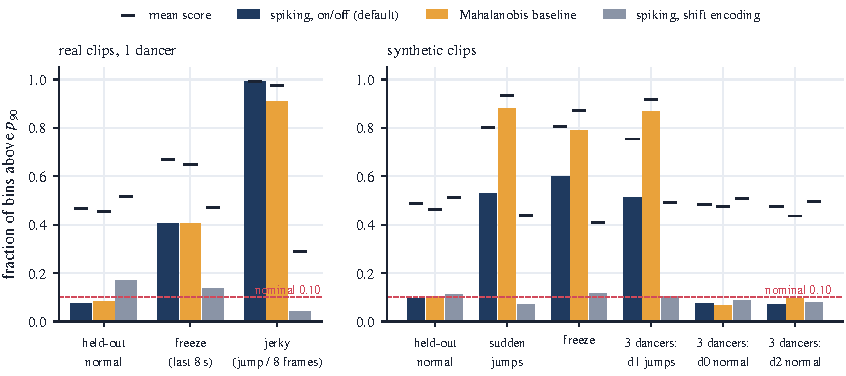
\includegraphics[width=\linewidth]{figures/out/scorer.pdf}
  \caption[Scorer comparison]{\textbf{Fraction of bins above $p_{90}$} for the three scorers (bars) with the mean score (black ticks); data from \cref{tab:scorer-real,tab:scorer-synth}. Dashed: the nominal 0.10 for normal clips.}
  \label{fig:scorer}
\end{figure}

\paragraph{Findings.} (i) Our five cabin takes (\TakeEScore{} to \TakeAScore{}, 0.3 to 1.5\% flagged) and the public clip (\SoloScore{}, \SoloAbove{} flagged) are all in the default model's training set, so they score at or below the clean median, as training data should. Held out, the author measures 0.471 / 0.033 for the public performer, near the calibrated 0.5 / 0.10, and 0.192 / 0.003 for one cabin take; with models trained only on takes from our room, 8 of 9 deliberately bad takes are flagged, with clean and bad takes filmed 30 minutes apart. Calibration needs clean clips from the room being scored. An earlier version of this paper scored with pose boxes on models trained on vertical strips, which inflated the public clip to 0.84; all numbers here use the regions of training. (ii) In the author's controlled tests the on/off spiking scorer and the Mahalanobis baseline are about equal: the spiking scorer is slightly better on real clips (0.992 versus 0.911 on jerky motion), the baseline clearly better on synthetic ones (0.880 versus 0.529 on jumps). (iii) The original shift encoding fails as predicted in \cref{sec:scorer}: it scores both abnormal real clips \emph{below} the normal one. (iv) The weights do not specialise. After training they are nearly equal, standard deviation 0.017 to 0.019 around 0.25 (\cref{tab:diag}), so the score approximates a leaky sum of absolute deviations, the same signal as the baseline with memory. The sparsity mechanisms made the network work, but not learn. (v) No scorer detects a 3$\times$ speed-up; that clip was removed from the tables rather than averaged away. (vi) The sync score separates a jumping synthetic dancer (0.538) from two dancers in step (0.244 each); it is untested on real multi-dancer clips.

\subsection{Robot ears}
\label{sec:exp-ears}

On a real \SnoreSeconds\,s snoring recording the simulated cochlea emits \SnoreEvCount{} events over \SnoreChannels{} channels, \SnoreEvRate{}k events per second (\cref{fig:snore}). The breathing analysis finds \SnoreOnsets{} snore onsets and a cadence of \SnoreBpm{} breaths per minute with autocorrelation strength \SnoreCadence; it reports \SnorePauses{} long pauses. These are signal-processing estimates on one recording, not a clinical measurement, and the robot's reaction is scripted.

\begin{figure}[tbp]
  \centering
  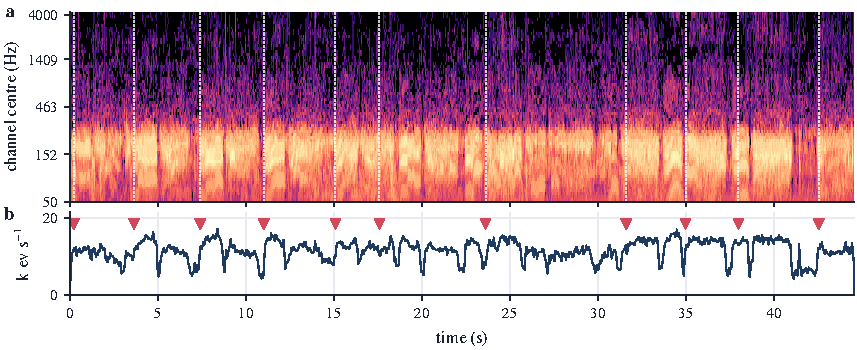
\includegraphics[width=\linewidth]{figures/out/snore.pdf}
  \caption[The robot's ears: simulated cochleagram of a snore]{\textbf{The robot's ears.} (a) Cochleagram of simulated address events, 50\,ms bins, log count; dashed lines: detected snore onsets. (b) Total event rate; triangles: detected snore onsets. The input recording is real; the cochlea and its events are simulated.}
  \label{fig:snore}
\end{figure}

\subsection{From replay to physics}
\label{sec:exp-physics}

After \PhysIter{} PPO iterations, about \PhysTrainMin{} minutes on one \PhysGPU{}, we roll the policy out once over the whole take in simulation, deterministically, with no resets. The G1 completes all \PhysSeconds\,s without falling (fall: pelvis below 0.45\,m or torso tilt beyond 60\textdegree). Its pelvis never drops below \PhysMinHeight\,m, the torso stays upright (minimum cosine to vertical \PhysUpright), and the base drifts at most \PhysDrift\,cm. Tracked bodies stay within \PhysBodyErrCm\,cm of the reference on average; joint angle error is \PhysJointRmse\,rad overall and \PhysArmRmse\,rad on the arms, where the macarena happens. The reference was kinematically feasible to begin with (standing legs, arm motion only), which is the easy case; a jump, a turn or hip motion would be harder. \Cref{fig:physics} shows five frames of the rollout. This is a result in simulation. Sim-to-real transfer to a physical G1 needs domain randomisation and a safety review we have not done.

\begin{figure}[tbp]
  \centering
  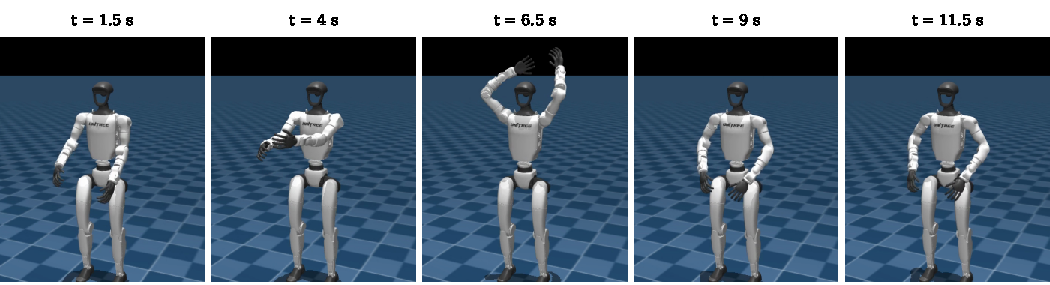
\includegraphics[width=\linewidth]{figures/out/physics_strip.pdf}
  \caption[The G1 dancing our take in simulated physics]{\textbf{From replay to physics.} The PPO tracking policy (\cref{eq:track-reward,eq:ppo}) after \PhysIter{} iterations, rolled out once over cabin take 3 in simulated rigid-body physics. The robot balances on its own feet and applies joint torques; it does not fall. Simulated physics; not run on a real robot.}
  \label{fig:physics}
\end{figure}

\subsection{Runtime}
\label{sec:exp-runtime}

\begin{table}[tbp]
\centering
\caption{\textbf{Runtime} on one MacBook CPU, single runs. Left: stages timed by \file{figures/time\_stages.py} on cabin take 3 (\TakeCSec\,s, 286 frames). Right: the one-command run on the \SoloSeconds\,s public clip, from the run log.}
\label{tab:runtime}
\small
\begin{tabular}{@{}l r l r@{}}
\toprule
\multicolumn{2}{@{}l}{Cabin take 3, per stage} & \multicolumn{2}{l@{}}{Public clip, one command} \\
\cmidrule(r){1-2}\cmidrule(l){3-4}
Pose, MediaPipe (\PoseFps{} frames/s) & \TPose\,s & Pose & \TSoloPose\,s \\
Retargeting (IK), no render & \TRobot\,s & Robot, with render & \TSoloRobot\,s \\
Events, eventify, simulated & \TEvents\,s & Scoring & \TSoloScore\,s \\
Steam veil, one level & \TSteam\,s & Viewer & \TSoloViewer\,s \\
& & Steam sweep, 6 levels & \TSoloSteam\,s \\
\bottomrule
\end{tabular}
\end{table}

Pose estimation dominates every run except the steam sweep, which re-runs pose once per level (\cref{tab:runtime}). The \SoloSeconds\,s clip takes about 40\,s without the sweep and about 3.6 minutes with it. The pipeline meets our rule of under three minutes per short clip end to end, but the six-level sweep alone breaks it; a three-level sweep would not.

\section{Limitations and Threats to Validity}
\label{sec:limits}

\begin{itemize}
  \item \textbf{Construct validity.} The steam curve measures the response of one pose model to one analytic veil. Real steam has different spectra, droplet sizes, condensation on the lens and a photographer who is very warm. The veil is not fitted to real steam, and the sweep is reported on one clip.
  \item \textbf{External validity.} Five takes of one team member in one room, and one public clip. Our scored clips are in the scorer's training set (\cref{tab:cabin}); the held-out numbers are the scorer author's and come from a handful of clips. $n$ is small everywhere.
  \item \textbf{Simulated sensors.} The event stream is an idealised frame-difference model with no noise, latency or refractory period; at 25 fps its timing is coarse. It is not sensor data and we do not call it that. The cochlea is equally idealised.
  \item \textbf{The robot.} The G1 replay is kinematic. It ignores balance, torque limits, self-collision and the legs, and does not recover palm orientation. The macarena's palm flip is therefore not performed. The physics policy of \cref{sec:exp-physics} addresses balance and torque limits in simulation only, on an easy, standing reference; it has not run on hardware.
  \item \textbf{The scorer.} Its weights do not specialise and STDP adds little; the baseline is as good. Its percentiles shift between rooms. No scorer detects a 3$\times$ speed-up. Real multi-dancer clips are untested.
  \item \textbf{Internal validity.} The controlled scorer tables were produced by their author and reproduced without a re-run. Runtimes come from one machine and one run each.
  \item \textbf{Researcher degrees of freedom.} We chose the steam levels before seeing the curve and did not tune the veil afterwards; but we chose the veil.
  \item \textbf{Conflict of interest.} The authors stand to win a macarena.
\end{itemize}

\section{Broader Impact}
\label{sec:impact}

The most likely deployment of \vlma{} is a wedding. A system that scores each dancer's unusualness in real time could be used to identify the uncle who is off the beat. We recommend that scores be shown only to the dancer concerned, and never to the uncle. More seriously: the pipeline turns video of people into derived data. We keep other people's raw video out of the repository unless they agreed, commit only derived pose and events, process audio in memory, and run everything locally. The event stream, the pose and the cochlea are lossy enough that we consider the derived files low-risk, but they are still derived from people and are treated as such. Pose models perform unevenly across bodies, clothing and lighting; a steam-like degradation is one of many conditions under which they fail, and failure falls on whoever is least visible. Finally, a humanoid that performs the macarena may increase the number of macarenas in the world. We have not studied this risk.

\section{Conclusion}
\label{sec:conclusion}

A phone, a laptop and an afternoon are enough to turn a macarena into a labelled humanoid episode with simulated events, estimated pose and a kinematic replay that follows the arms through every move except the palm flip. The weak links are measurable. Perception fails between \LossSThirty\% and \LossSForty\% loss of light in simulated steam. The spiking scorer is no better than a Mahalanobis distance, and it needs clean clips from the room it scores. A tracking policy trained in minutes on one GPU turns the replay into a balanced, physically simulated dance. The robot cannot yet survive a sauna. Neither could we.

\paragraph{Acknowledgements.} We thank the cabin for its television and the team member who danced the macarena five times.

{\small
\bibliographystyle{unsrtnat}
\bibliography{references}
}

\clearpage
\appendix
\section{Reproducibility Checklist}
\label{app:repro}

\begin{small}
\begin{tabularx}{\linewidth}{@{}>{\raggedright\arraybackslash}X >{\raggedright\arraybackslash}p{5.2cm}@{}}
\toprule
Item & Status \\
\midrule
Every figure is generated by a script in \file{paper/figures/} from files in \file{episodes/} & yes \\
Every number in the text comes from \file{paper/numbers.tex}, generated by \file{figures/make\_numbers.py} & yes, except the controlled scorer tables, copied verbatim \\
Fixed random seeds (steam noise seed 0, event subsample seed 0) & yes \\
One command reproduces an episode from a clip & yes (\cref{alg:run}) \\
Code, assets and versions listed & yes, repository README \\
Raw video of third parties in the repository & no \\
Simulated streams labelled as simulated in files, figures and video & yes \\
Hardware & one MacBook, CPU only \\
Error bars and repeated runs & no: single runs; five takes of one dancer \\
Statistical significance tests & no \\
\bottomrule
\end{tabularx}
\end{small}

\paragraph{Rebuilding this paper.} \texttt{cd paper \&\& ./build.sh} regenerates all figures and \file{numbers.tex} from the episode folders, then runs \texttt{latexmk}. \texttt{VLMA\_EPISODE=<clip\_id> ./build.sh} points every figure and number at another episode.

\section{Scorer Controlled Results}
\label{app:scorer}

The scorer author's synthetic benchmark and network diagnostics, copied from the scorer's progress log and not re-run by us.

\begin{table}[h]
\centering
\caption{\textbf{Synthetic clips.} Training: 7 synthetic normal clips. Mean score / fraction above $p_{90}$.}
\label{tab:scorer-synth}
\small
\begin{tabular}{@{}l c c c@{}}
\toprule
Clip & Baseline (Mahalanobis) & Spiking, shift encoding & Spiking, on/off (default) \\
\midrule
Held-out normal & 0.462 / 0.103 & 0.513 / 0.112 & 0.489 / 0.095 \\
Sudden jumps & 0.934 / \textbf{0.880} & 0.437 / 0.070 & 0.800 / 0.529 \\
Freeze & 0.872 / \textbf{0.789} & 0.409 / 0.116 & 0.806 / 0.599 \\
Three dancers: dancer 1, jumps & 0.918 / \textbf{0.868} & 0.493 / 0.103 & 0.754 / 0.512 \\
Three dancers: dancer 0, normal & 0.475 / 0.066 & 0.510 / 0.087 & 0.485 / 0.074 \\
Three dancers: dancer 2, normal & 0.436 / 0.095 & 0.495 / 0.079 & 0.474 / 0.070 \\
\bottomrule
\end{tabular}
\end{table}

\begin{table}[h]
\centering
\caption{\textbf{Spiking network diagnostics} on real training features, before and after the three sparsity changes, and \textbf{feature ablation} for the baseline on real clips (mean / fraction above $p_{90}$). From the scorer's progress log.}
\label{tab:diag}
\small
\begin{tabular}{@{}l c c@{}}
\toprule
Diagnostic & Original network & With adaptive threshold, top-$k$, normalisation \\
\midrule
Hidden neurons firing per bin & 99.7\% (untrained) & 10.0\% \\
Output neurons firing per bin & 100\% (untrained) & 9.7--10.0\% \\
Mean input current, hidden (threshold 1.0) & 1.62 & -- \\
Weights after training & layer 2 all equal & s.d.\ 0.017--0.019 around 0.25 \\
\bottomrule
\end{tabular}

\vspace{6pt}
\begin{tabular}{@{}l c c c@{}}
\toprule
Real clip & 13 features & 26 (with deltas) & 26, self-centred box, relative rate \\
\midrule
Held-out normal & 0.392 / 0.040 & 0.420 / 0.074 & 0.455 / 0.082 \\
Abnormal: freeze & 0.602 / 0.362 & 0.644 / 0.393 & 0.647 / 0.406 \\
Abnormal: jerky & 0.898 / 0.791 & 0.973 / 0.903 & 0.976 / 0.911 \\
\bottomrule
\end{tabular}
\end{table}

\clearpage
\section{Hyperparameters}
\label{app:hyper}

\begin{table}[h]
\centering
\caption{All hyperparameters, from the source code.}
\label{tab:hyper}
\small
\begin{tabular}{@{}l l l@{}}
\toprule
Stage & Parameter & Value \\
\midrule
Events & contrast threshold $C$; offset $\varepsilon$; sensor & 0.05; 1.0; $320{\times}180$ \\
& interpolated sub-frames (scorer training) & 3 \\
Pose & model; max poses; visibility gate & MediaPipe Pose Landmarker full; 3; 0.3 \\
Retargeting & solver; max evaluations; FD step & trust-region reflective; 35; $10^{-4}$ \\
& smoothing time constant $\tau$ & 55\,ms \\
Features & bin; running-mean window; box padding & 33\,ms; 300 bins ($\approx$10\,s); 15\% \\
Scorer & layers; $\beta$; base threshold & $52\to128\to32$; 0.9; 1.0 \\
& top-$k$ fraction; target rate $\rho^\ast$; $\eta$; min.\ threshold & 0.15; 0.10; 0.02; 0.05 \\
& $A_+$; $A_-$; trace $\tau$; weight decay; $W$ range & 0.005; 0.020; 20 steps; $10^{-3}$; $[0,1]$ \\
& epochs; rate-coding steps per bin; row sum & 6; 25; $0.25\,n_{\mathrm{in}}$ \\
& ZCA eigenvalue floor; on/off gain $g$; threshold & $10^{-3}$; 2.0; $p_{90}$ \\
Baseline & covariance ridge & $10^{-3}$ \\
Sync & correlation window & 2\,s \\
Steam & $\beta$ range; airlight; noise grids; seed & $[0,5]$; (235, 233, 228); $8^2,16^2,32^2$; 0 \\
& blur width; puff cycle & $0.3+0.35\beta$ px; 9\,s \\
Cochlea & channels; band; filter order; envelope low-pass & 64; 50\,Hz--4\,kHz; 2; 200\,Hz \\
& envelope rate; $\theta$; refractory & 4\,kHz; \SnoreTheta; 1\,ms \\
\bottomrule
\end{tabular}
\end{table}

\section{Contract Formats}
\label{app:contract}

\begin{small}
\begin{tabularx}{\linewidth}{@{}l X@{}}
\toprule
File & Format \\
\midrule
\file{events.h5} & HDF5 group \file{/events}: \file{xs}, \file{ys} int16; \file{ts} int64 \textmu s; \file{ps} int8 (0 OFF, 1 ON); attribute \file{sensor\_shape} $=(H,W)$, $W\le320$. DVS128 Gesture layout~\cite{amir2017gesture}. \\
\file{audio\_events.h5} & as above with $H=1$, $W=64$ channels; attributes \file{channel\_hz}, \file{theta}, \file{refractory\_us}, \file{simulated}=true, \file{method}. \\
\file{poses.npy} & float32 $(F,D,17,3)$, COCO order, $x,y$ in source pixels, confidence; missing joint has confidence 0. \\
\file{pose3d.npz} & \file{world} $(F,D,33,3)$ metres, \file{vis} $(F,D,33)$, \file{image}, \file{fps}. \\
\file{robot.npz} & \file{qpos} $(F,36)$, \file{joint\_names}, \file{joint\_qposadr}, \file{limit\_hits} $(F)$, \file{fps}, torso axes. \\
\file{scores.npy} & float32 $(B,D)$ in $[0,1]$; bin $k$ covers $[33k, 33(k{+}1))$\,ms from the first frame. \\
\file{scores\_meta.json} & \file{bin\_ms}, \file{bins}, sensor size, \file{scorer}, \file{threshold}, \file{sync}, ranking. \\
\file{steam\_metrics.csv} & \file{level}, \file{mean\_transmittance}, per dancer \file{detected\_fraction}, \file{mean\_confidence}, \file{mean\_keypoint\_drift\_px}, \file{unusualness\_mean}. \\
\bottomrule
\end{tabularx}
\end{small}

\end{document}
